\documentclass{article}




\usepackage[final]{neurips_2023}









%%%%% NEW MATH DEFINITIONS %%%%%

\usepackage{amsmath,amsfonts,bm}

% Mark sections of captions for referring to divisions of figures
\newcommand{\figleft}{{\em (Left)}}
\newcommand{\figcenter}{{\em (Center)}}
\newcommand{\figright}{{\em (Right)}}
\newcommand{\figtop}{{\em (Top)}}
\newcommand{\figbottom}{{\em (Bottom)}}
\newcommand{\captiona}{{\em (a)}}
\newcommand{\captionb}{{\em (b)}}
\newcommand{\captionc}{{\em (c)}}
\newcommand{\captiond}{{\em (d)}}

% Highlight a newly defined term
\newcommand{\newterm}[1]{{\bf #1}}


% Figure reference, lower-case.
\def\figref#1{figure~\ref{#1}}
% Figure reference, capital. For start of sentence
\def\Figref#1{Figure~\ref{#1}}
\def\twofigref#1#2{figures \ref{#1} and \ref{#2}}
\def\quadfigref#1#2#3#4{figures \ref{#1}, \ref{#2}, \ref{#3} and \ref{#4}}
% Section reference, lower-case.
\def\secref#1{section~\ref{#1}}
% Section reference, capital.
\def\Secref#1{Section~\ref{#1}}
% Reference to two sections.
\def\twosecrefs#1#2{sections \ref{#1} and \ref{#2}}
% Reference to three sections.
\def\secrefs#1#2#3{sections \ref{#1}, \ref{#2} and \ref{#3}}
% Reference to an equation, lower-case.
\def\eqref#1{equation~\ref{#1}}
% Reference to an equation, upper case
\def\Eqref#1{Equation~\ref{#1}}
% A raw reference to an equation---avoid using if possible
\def\plaineqref#1{\ref{#1}}
% Reference to a chapter, lower-case.
\def\chapref#1{chapter~\ref{#1}}
% Reference to an equation, upper case.
\def\Chapref#1{Chapter~\ref{#1}}
% Reference to a range of chapters
\def\rangechapref#1#2{chapters\ref{#1}--\ref{#2}}
% Reference to an algorithm, lower-case.
\def\algref#1{algorithm~\ref{#1}}
% Reference to an algorithm, upper case.
\def\Algref#1{Algorithm~\ref{#1}}
\def\twoalgref#1#2{algorithms \ref{#1} and \ref{#2}}
\def\Twoalgref#1#2{Algorithms \ref{#1} and \ref{#2}}
% Reference to a part, lower case
\def\partref#1{part~\ref{#1}}
% Reference to a part, upper case
\def\Partref#1{Part~\ref{#1}}
\def\twopartref#1#2{parts \ref{#1} and \ref{#2}}

\def\ceil#1{\lceil #1 \rceil}
\def\floor#1{\lfloor #1 \rfloor}
\def\1{\bm{1}}
\newcommand{\train}{\mathcal{D}}
\newcommand{\valid}{\mathcal{D_{\mathrm{valid}}}}
\newcommand{\test}{\mathcal{D_{\mathrm{test}}}}

\def\eps{{\epsilon}}


% Random variables
\def\reta{{\textnormal{$\eta$}}}
\def\ra{{\textnormal{a}}}
\def\rb{{\textnormal{b}}}
\def\rc{{\textnormal{c}}}
\def\rd{{\textnormal{d}}}
\def\re{{\textnormal{e}}}
\def\rf{{\textnormal{f}}}
\def\rg{{\textnormal{g}}}
\def\rh{{\textnormal{h}}}
\def\ri{{\textnormal{i}}}
\def\rj{{\textnormal{j}}}
\def\rk{{\textnormal{k}}}
\def\rl{{\textnormal{l}}}
% rm is already a command, just don't name any random variables m
\def\rn{{\textnormal{n}}}
\def\ro{{\textnormal{o}}}
\def\rp{{\textnormal{p}}}
\def\rq{{\textnormal{q}}}
\def\rr{{\textnormal{r}}}
\def\rs{{\textnormal{s}}}
\def\rt{{\textnormal{t}}}
\def\ru{{\textnormal{u}}}
\def\rv{{\textnormal{v}}}
\def\rw{{\textnormal{w}}}
\def\rx{{\textnormal{x}}}
\def\ry{{\textnormal{y}}}
\def\rz{{\textnormal{z}}}

% Random vectors
\def\rvepsilon{{\mathbf{\epsilon}}}
\def\rvtheta{{\mathbf{\theta}}}
\def\rva{{\mathbf{a}}}
\def\rvb{{\mathbf{b}}}
\def\rvc{{\mathbf{c}}}
\def\rvd{{\mathbf{d}}}
\def\rve{{\mathbf{e}}}
\def\rvf{{\mathbf{f}}}
\def\rvg{{\mathbf{g}}}
\def\rvh{{\mathbf{h}}}
\def\rvu{{\mathbf{i}}}
\def\rvj{{\mathbf{j}}}
\def\rvk{{\mathbf{k}}}
\def\rvl{{\mathbf{l}}}
\def\rvm{{\mathbf{m}}}
\def\rvn{{\mathbf{n}}}
\def\rvo{{\mathbf{o}}}
\def\rvp{{\mathbf{p}}}
\def\rvq{{\mathbf{q}}}
\def\rvr{{\mathbf{r}}}
\def\rvs{{\mathbf{s}}}
\def\rvt{{\mathbf{t}}}
\def\rvu{{\mathbf{u}}}
\def\rvv{{\mathbf{v}}}
\def\rvw{{\mathbf{w}}}
\def\rvx{{\mathbf{x}}}
\def\rvy{{\mathbf{y}}}
\def\rvz{{\mathbf{z}}}

% Elements of random vectors
\def\erva{{\textnormal{a}}}
\def\ervb{{\textnormal{b}}}
\def\ervc{{\textnormal{c}}}
\def\ervd{{\textnormal{d}}}
\def\erve{{\textnormal{e}}}
\def\ervf{{\textnormal{f}}}
\def\ervg{{\textnormal{g}}}
\def\ervh{{\textnormal{h}}}
\def\ervi{{\textnormal{i}}}
\def\ervj{{\textnormal{j}}}
\def\ervk{{\textnormal{k}}}
\def\ervl{{\textnormal{l}}}
\def\ervm{{\textnormal{m}}}
\def\ervn{{\textnormal{n}}}
\def\ervo{{\textnormal{o}}}
\def\ervp{{\textnormal{p}}}
\def\ervq{{\textnormal{q}}}
\def\ervr{{\textnormal{r}}}
\def\ervs{{\textnormal{s}}}
\def\ervt{{\textnormal{t}}}
\def\ervu{{\textnormal{u}}}
\def\ervv{{\textnormal{v}}}
\def\ervw{{\textnormal{w}}}
\def\ervx{{\textnormal{x}}}
\def\ervy{{\textnormal{y}}}
\def\ervz{{\textnormal{z}}}

% Random matrices
\def\rmA{{\mathbf{A}}}
\def\rmB{{\mathbf{B}}}
\def\rmC{{\mathbf{C}}}
\def\rmD{{\mathbf{D}}}
\def\rmE{{\mathbf{E}}}
\def\rmF{{\mathbf{F}}}
\def\rmG{{\mathbf{G}}}
\def\rmH{{\mathbf{H}}}
\def\rmI{{\mathbf{I}}}
\def\rmJ{{\mathbf{J}}}
\def\rmK{{\mathbf{K}}}
\def\rmL{{\mathbf{L}}}
\def\rmM{{\mathbf{M}}}
\def\rmN{{\mathbf{N}}}
\def\rmO{{\mathbf{O}}}
\def\rmP{{\mathbf{P}}}
\def\rmQ{{\mathbf{Q}}}
\def\rmR{{\mathbf{R}}}
\def\rmS{{\mathbf{S}}}
\def\rmT{{\mathbf{T}}}
\def\rmU{{\mathbf{U}}}
\def\rmV{{\mathbf{V}}}
\def\rmW{{\mathbf{W}}}
\def\rmX{{\mathbf{X}}}
\def\rmY{{\mathbf{Y}}}
\def\rmZ{{\mathbf{Z}}}

% Elements of random matrices
\def\ermA{{\textnormal{A}}}
\def\ermB{{\textnormal{B}}}
\def\ermC{{\textnormal{C}}}
\def\ermD{{\textnormal{D}}}
\def\ermE{{\textnormal{E}}}
\def\ermF{{\textnormal{F}}}
\def\ermG{{\textnormal{G}}}
\def\ermH{{\textnormal{H}}}
\def\ermI{{\textnormal{I}}}
\def\ermJ{{\textnormal{J}}}
\def\ermK{{\textnormal{K}}}
\def\ermL{{\textnormal{L}}}
\def\ermM{{\textnormal{M}}}
\def\ermN{{\textnormal{N}}}
\def\ermO{{\textnormal{O}}}
\def\ermP{{\textnormal{P}}}
\def\ermQ{{\textnormal{Q}}}
\def\ermR{{\textnormal{R}}}
\def\ermS{{\textnormal{S}}}
\def\ermT{{\textnormal{T}}}
\def\ermU{{\textnormal{U}}}
\def\ermV{{\textnormal{V}}}
\def\ermW{{\textnormal{W}}}
\def\ermX{{\textnormal{X}}}
\def\ermY{{\textnormal{Y}}}
\def\ermZ{{\textnormal{Z}}}

% Vectors
\def\vzero{{\bm{0}}}
\def\vone{{\bm{1}}}
\def\vmu{{\bm{\mu}}}
\def\vtheta{{\bm{\theta}}}
\def\va{{\bm{a}}}
\def\vb{{\bm{b}}}
\def\vc{{\bm{c}}}
\def\vd{{\bm{d}}}
\def\ve{{\bm{e}}}
\def\vf{{\bm{f}}}
\def\vg{{\bm{g}}}
\def\vh{{\bm{h}}}
\def\vi{{\bm{i}}}
\def\vj{{\bm{j}}}
\def\vk{{\bm{k}}}
\def\vl{{\bm{l}}}
\def\vm{{\bm{m}}}
\def\vn{{\bm{n}}}
\def\vo{{\bm{o}}}
\def\vp{{\bm{p}}}
\def\vq{{\bm{q}}}
\def\vr{{\bm{r}}}
\def\vs{{\bm{s}}}
\def\vt{{\bm{t}}}
\def\vu{{\bm{u}}}
\def\vv{{\bm{v}}}
\def\vw{{\bm{w}}}
\def\vx{{\bm{x}}}
\def\vy{{\bm{y}}}
\def\vz{{\bm{z}}}

% Elements of vectors
\def\evalpha{{\alpha}}
\def\evbeta{{\beta}}
\def\evepsilon{{\epsilon}}
\def\evlambda{{\lambda}}
\def\evomega{{\omega}}
\def\evmu{{\mu}}
\def\evpsi{{\psi}}
\def\evsigma{{\sigma}}
\def\evtheta{{\theta}}
\def\eva{{a}}
\def\evb{{b}}
\def\evc{{c}}
\def\evd{{d}}
\def\eve{{e}}
\def\evf{{f}}
\def\evg{{g}}
\def\evh{{h}}
\def\evi{{i}}
\def\evj{{j}}
\def\evk{{k}}
\def\evl{{l}}
\def\evm{{m}}
\def\evn{{n}}
\def\evo{{o}}
\def\evp{{p}}
\def\evq{{q}}
\def\evr{{r}}
\def\evs{{s}}
\def\evt{{t}}
\def\evu{{u}}
\def\evv{{v}}
\def\evw{{w}}
\def\evx{{x}}
\def\evy{{y}}
\def\evz{{z}}

% Matrix
\def\mA{{\bm{A}}}
\def\mB{{\bm{B}}}
\def\mC{{\bm{C}}}
\def\mD{{\bm{D}}}
\def\mE{{\bm{E}}}
\def\mF{{\bm{F}}}
\def\mG{{\bm{G}}}
\def\mH{{\bm{H}}}
\def\mI{{\bm{I}}}
\def\mJ{{\bm{J}}}
\def\mK{{\bm{K}}}
\def\mL{{\bm{L}}}
\def\mM{{\bm{M}}}
\def\mN{{\bm{N}}}
\def\mO{{\bm{O}}}
\def\mP{{\bm{P}}}
\def\mQ{{\bm{Q}}}
\def\mR{{\bm{R}}}
\def\mS{{\bm{S}}}
\def\mT{{\bm{T}}}
\def\mU{{\bm{U}}}
\def\mV{{\bm{V}}}
\def\mW{{\bm{W}}}
\def\mX{{\bm{X}}}
\def\mY{{\bm{Y}}}
\def\mZ{{\bm{Z}}}
\def\mBeta{{\bm{\beta}}}
\def\mPhi{{\bm{\Phi}}}
\def\mLambda{{\bm{\Lambda}}}
\def\mSigma{{\bm{\Sigma}}}

% Tensor
\DeclareMathAlphabet{\mathsfit}{\encodingdefault}{\sfdefault}{m}{sl}
\SetMathAlphabet{\mathsfit}{bold}{\encodingdefault}{\sfdefault}{bx}{n}
\newcommand{\tens}[1]{\bm{\mathsfit{#1}}}
\def\tA{{\tens{A}}}
\def\tB{{\tens{B}}}
\def\tC{{\tens{C}}}
\def\tD{{\tens{D}}}
\def\tE{{\tens{E}}}
\def\tF{{\tens{F}}}
\def\tG{{\tens{G}}}
\def\tH{{\tens{H}}}
\def\tI{{\tens{I}}}
\def\tJ{{\tens{J}}}
\def\tK{{\tens{K}}}
\def\tL{{\tens{L}}}
\def\tM{{\tens{M}}}
\def\tN{{\tens{N}}}
\def\tO{{\tens{O}}}
\def\tP{{\tens{P}}}
\def\tQ{{\tens{Q}}}
\def\tR{{\tens{R}}}
\def\tS{{\tens{S}}}
\def\tT{{\tens{T}}}
\def\tU{{\tens{U}}}
\def\tV{{\tens{V}}}
\def\tW{{\tens{W}}}
\def\tX{{\tens{X}}}
\def\tY{{\tens{Y}}}
\def\tZ{{\tens{Z}}}


% Graph
\def\gA{{\mathcal{A}}}
\def\gB{{\mathcal{B}}}
\def\gC{{\mathcal{C}}}
\def\gD{{\mathcal{D}}}
\def\gE{{\mathcal{E}}}
\def\gF{{\mathcal{F}}}
\def\gG{{\mathcal{G}}}
\def\gH{{\mathcal{H}}}
\def\gI{{\mathcal{I}}}
\def\gJ{{\mathcal{J}}}
\def\gK{{\mathcal{K}}}
\def\gL{{\mathcal{L}}}
\def\gM{{\mathcal{M}}}
\def\gN{{\mathcal{N}}}
\def\gO{{\mathcal{O}}}
\def\gP{{\mathcal{P}}}
\def\gQ{{\mathcal{Q}}}
\def\gR{{\mathcal{R}}}
\def\gS{{\mathcal{S}}}
\def\gT{{\mathcal{T}}}
\def\gU{{\mathcal{U}}}
\def\gV{{\mathcal{V}}}
\def\gW{{\mathcal{W}}}
\def\gX{{\mathcal{X}}}
\def\gY{{\mathcal{Y}}}
\def\gZ{{\mathcal{Z}}}

% Sets
\def\sA{{\mathbb{A}}}
\def\sB{{\mathbb{B}}}
\def\sC{{\mathbb{C}}}
\def\sD{{\mathbb{D}}}
% Don't use a set called E, because this would be the same as our symbol
% for expectation.
\def\sF{{\mathbb{F}}}
\def\sG{{\mathbb{G}}}
\def\sH{{\mathbb{H}}}
\def\sI{{\mathbb{I}}}
\def\sJ{{\mathbb{J}}}
\def\sK{{\mathbb{K}}}
\def\sL{{\mathbb{L}}}
\def\sM{{\mathbb{M}}}
\def\sN{{\mathbb{N}}}
\def\sO{{\mathbb{O}}}
\def\sP{{\mathbb{P}}}
\def\sQ{{\mathbb{Q}}}
\def\sR{{\mathbb{R}}}
\def\sS{{\mathbb{S}}}
\def\sT{{\mathbb{T}}}
\def\sU{{\mathbb{U}}}
\def\sV{{\mathbb{V}}}
\def\sW{{\mathbb{W}}}
\def\sX{{\mathbb{X}}}
\def\sY{{\mathbb{Y}}}
\def\sZ{{\mathbb{Z}}}

% Entries of a matrix
\def\emLambda{{\Lambda}}
\def\emA{{A}}
\def\emB{{B}}
\def\emC{{C}}
\def\emD{{D}}
\def\emE{{E}}
\def\emF{{F}}
\def\emG{{G}}
\def\emH{{H}}
\def\emI{{I}}
\def\emJ{{J}}
\def\emK{{K}}
\def\emL{{L}}
\def\emM{{M}}
\def\emN{{N}}
\def\emO{{O}}
\def\emP{{P}}
\def\emQ{{Q}}
\def\emR{{R}}
\def\emS{{S}}
\def\emT{{T}}
\def\emU{{U}}
\def\emV{{V}}
\def\emW{{W}}
\def\emX{{X}}
\def\emY{{Y}}
\def\emZ{{Z}}
\def\emSigma{{\Sigma}}

% entries of a tensor
% Same font as tensor, without \bm wrapper
\newcommand{\etens}[1]{\mathsfit{#1}}
\def\etLambda{{\etens{\Lambda}}}
\def\etA{{\etens{A}}}
\def\etB{{\etens{B}}}
\def\etC{{\etens{C}}}
\def\etD{{\etens{D}}}
\def\etE{{\etens{E}}}
\def\etF{{\etens{F}}}
\def\etG{{\etens{G}}}
\def\etH{{\etens{H}}}
\def\etI{{\etens{I}}}
\def\etJ{{\etens{J}}}
\def\etK{{\etens{K}}}
\def\etL{{\etens{L}}}
\def\etM{{\etens{M}}}
\def\etN{{\etens{N}}}
\def\etO{{\etens{O}}}
\def\etP{{\etens{P}}}
\def\etQ{{\etens{Q}}}
\def\etR{{\etens{R}}}
\def\etS{{\etens{S}}}
\def\etT{{\etens{T}}}
\def\etU{{\etens{U}}}
\def\etV{{\etens{V}}}
\def\etW{{\etens{W}}}
\def\etX{{\etens{X}}}
\def\etY{{\etens{Y}}}
\def\etZ{{\etens{Z}}}

% The true underlying data generating distribution
\newcommand{\pdata}{p_{\rm{data}}}
% The empirical distribution defined by the training set
\newcommand{\ptrain}{\hat{p}_{\rm{data}}}
\newcommand{\Ptrain}{\hat{P}_{\rm{data}}}
% The model distribution
\newcommand{\pmodel}{p_{\rm{model}}}
\newcommand{\Pmodel}{P_{\rm{model}}}
\newcommand{\ptildemodel}{\tilde{p}_{\rm{model}}}
% Stochastic autoencoder distributions
\newcommand{\pencode}{p_{\rm{encoder}}}
\newcommand{\pdecode}{p_{\rm{decoder}}}
\newcommand{\precons}{p_{\rm{reconstruct}}}

\newcommand{\laplace}{\mathrm{Laplace}} % Laplace distribution

\newcommand{\E}{\mathbb{E}}
\newcommand{\Ls}{\mathcal{L}}
\newcommand{\R}{\mathbb{R}}
\newcommand{\emp}{\tilde{p}}
\newcommand{\lr}{\alpha}
\newcommand{\reg}{\lambda}
\newcommand{\rect}{\mathrm{rectifier}}
\newcommand{\softmax}{\mathrm{softmax}}
\newcommand{\sigmoid}{\sigma}
\newcommand{\softplus}{\zeta}
\newcommand{\KL}{D_{\mathrm{KL}}}
\newcommand{\Var}{\mathrm{Var}}
\newcommand{\standarderror}{\mathrm{SE}}
\newcommand{\Cov}{\mathrm{Cov}}
% Wolfram Mathworld says $L^2$ is for function spaces and $\ell^2$ is for vectors
% But then they seem to use $L^2$ for vectors throughout the site, and so does
% wikipedia.
\newcommand{\normlzero}{L^0}
\newcommand{\normlone}{L^1}
\newcommand{\normltwo}{L^2}
\newcommand{\normlp}{L^p}
\newcommand{\normmax}{L^\infty}

\newcommand{\parents}{Pa} % See usage in notation.tex. Chosen to match Daphne's book.

\DeclareMathOperator*{\argmax}{arg\,max}
\DeclareMathOperator*{\argmin}{arg\,min}

\DeclareMathOperator{\sign}{sign}
\DeclareMathOperator{\Tr}{Tr}
\let\ab\allowbreak


\usepackage{hyperref}

\usepackage{lipsum}
\usepackage{latexsym}

\usepackage{graphicx}
\usepackage{subfigure}
\usepackage{booktabs} %
\usepackage{lipsum}
\usepackage{amsmath}
\usepackage{amssymb, amsthm, latexsym}
\usepackage{multirow}
\usepackage{scalefnt}

\usepackage{enumitem}
\setlist[itemize]{leftmargin=*}
\setlist[enumerate]{leftmargin=*}

\usepackage{nicefrac}
\usepackage{xcolor}
\definecolor{OliveGreen}{rgb}{0,0.4,0}


\usepackage{algorithm}
\usepackage{algorithmic}

\renewcommand{\algorithmicrequire}{\textbf{Input:}}

\usepackage[T1]{fontenc}

\usepackage[utf8]{inputenc}

\usepackage{microtype}

\usepackage{inconsolata}


\newcommand{\newstuff}[1]{{\color{OliveGreen} #1}}


\title{Distributed Inference and Fine-tuning of Large~Language~Models Over~The~Internet}




\author{%
  Alexander Borzunov\thanks{Correspondence to: \texttt{borzunov.alexander@gmail.com}} \\
  HSE Univesity, Yandex \\
  \And
  Max Ryabinin \\
  HSE Univesity, Yandex \\
  \And
  Artem Chumachenko \\
  Neiro.ai \\
  \AND
  Dmitry Baranchuk \\
  Yandex \\
  \And
  Tim Dettmers \\
  University of Washington \\
  \And
  Younes Belkada \\
  Hugging Face \\
  \AND
  Pavel Samygin \\
  Yandex School of Data Analysis \\
  \And
  Colin Raffel \\
  Hugging Face
}


\begin{document}


\maketitle

\setcounter{footnote}{0}
\begin{abstract}

Large language models (LLMs) are useful in many NLP tasks and become more capable with size, with the best open-source models having over 50 billion parameters. 
However, using these 50B+ models requires high-end hardware, making them inaccessible to most researchers.
In this work, we investigate methods for cost-efficient inference and fine-tuning of LLMs, comparing local and distributed strategies. We observe that a \textit{large enough} model (50B+) can run efficiently even on geodistributed devices in a consumer-grade network.
This could allow running LLM efficiently by pooling together idle compute resources of multiple research groups and volunteers.
We address two open problems: (1) how to perform inference and fine-tuning reliably if any device can disconnect abruptly and (2) how to partition LLMs between devices with uneven hardware, joining and leaving at will.
In order to do that, we develop special fault-tolerant inference algorithms and load-balancing protocols that automatically assign devices to maximize the total system throughput.
We showcase these algorithms in \textsc{Petals}\footnote{\textsc{Petals} source code and documentation are available at \texttt{\href{https://petals.dev}{https://petals.dev}}}
~--- a decentralized system that runs Llama 2 (70B) and BLOOM (176B) over the Internet up to $10\times$ faster than offloading for interactive generation.
We evaluate the performance of our system in simulated conditions and a real-world setup spanning two continents.

\end{abstract}


\section{Introduction}\label{sect:intro}

Many recent influential discoveries in deep learning were enabled by the trend of scaling model and dataset size.
Over the last decade, computer vision has grown from training models with 60 million parameters~\cite{alexnet} on 1.3 million images~\cite{imagenet_cvpr09} to 15 times more parameters~\cite{Kolesnikov2020BigT} and 200 times more training data~\cite{jft-300m}. In natural language processing, the state-of-the-art language models~\cite{gpt3} with 175 billion parameters are trained on over 570GB of texts, and even this does not saturate the model quality~\cite{kaplan2020scaling}.
Training these large models can take years even with a top-of-the-line GPU server~\cite{gpt3costlambda}. As a result, researchers and practitioners often have to run distributed training with multiple machines~\cite{mlperf}.

The dominant approach to distributed deep learning is data-parallel training~\cite{valiant1990bridging}, where each worker processes a fraction of the training batch and then exchanges its gradients with peers. If done naïvely, the gradient exchange step can overload the network as the number of workers increases. To combat this issue, modern distributed training algorithms take advantage of communication-efficient protocols, such as all-reduce~\cite{bandwidth_optimal_allreduce}. These protocols 
allow workers to collectively compute the global average gradient with a constant communication overhead, regardless of the total number of peers.

However, this efficiency makes the protocols more fragile: if any single participant fails or takes too long to process its batch, all other nodes are stalled.
Therefore, scaling all-reduce protocols beyond a couple of servers requires specialized infrastructure with dedicated ultra-high bandwidth networking~\cite{mlperf}.
This kind of infrastructure is notoriously expensive compared to regular
GPU servers or preemptible cloud VMs (see Appendix~\ref{sect:cloud_costs} for details).

Hence, it is tempting to consider distributed training on cheap unreliable instances as a cost-efficient alternative. A similar scenario arises in federated learning~\cite{mcmahan2017communication}, where a single model is trained on heterogeneous devices due to privacy concerns.
In both scenarios, workers use a shared network, where both latency and bandwidth can vary drastically due to interference from other users~\cite{variability_azure}\nocite{variability_aws}. Furthermore, compute nodes are also subject to failure (or preemption) caused by factors beyond the protocol's control.

Running large-scale distributed training in these circumstances requires fault- and latency-tolerant algorithms~\cite{lian2017can,sgpush}. Most of these algorithms replace all-reduce averaging with \textbf{gossip}: each participant periodically downloads the latest parameters from their neighbors in a sparsely connected communication graph and averages the results. The updates gradually propagate through the graph over multiple rounds of averaging.
However, the communication required to perform gossip grows linearly with the number of neighbors. Hence, when scaling to hundreds of peers, decentralized SGD has to keep the communication graph sparse, slowing down the convergence.

In this work, we propose an alternative approach. Instead of relying on a predefined communication graph, participants dynamically organize themselves into groups using a fully decentralized matchmaking algorithm called \textbf{Moshpit All-Reduce}. This strategy allows us to use communication-efficient all-reduce protocols that significantly reduce the network load compared to gossip-based averaging, while still being able to operate in unreliable hardware and network conditions.

Our contributions can be summarized as follows:
\begin{itemize}
    \item We propose {\bf Moshpit All-Reduce} --- a novel decentralized averaging protocol for large-scale training with unreliable communication-constrained devices. According to our analysis, this method has exponential convergence rate independent of network topology and size.
    \item Armed with this averaging protocol, we develop {\bf Moshpit SGD} for distributed optimization. We derive convergence rates for this algorithm and establish its equivalence to Centralized (Local) SGD in terms of iteration complexity under realistic assumptions.
    \item Our experiments demonstrate that Moshpit All-Reduce is significantly more efficient under network latency in realistic conditions. In particular, we train ResNet-50 on ImageNet to 75\% accuracy 1.3 times faster than existing decentralized training algorithms and pretrain ALBERT-large 1.5 times faster on preemptible cloud VMs.\footnote{Implementation and code of experiments are at \href{https://github.com/yandex-research/moshpit-sgd}{\texttt{github.com/yandex-research/moshpit-sgd}}.}
\end{itemize}

\section{Preliminaries: Ensembles and Distillation}

We view ensembles within a Bayesian framework where the model parameters $\bm{\theta}$ are random variables over which a prior distribution ${\tt p}(\bm{\theta})$ is placed. The posterior distribution ${\tt p}(\bm{\theta}|\mathcal{D})$ is obtained via Bayes' rule:
\begin{empheq}{align}
\begin{split}
  {\tt p}(\bm{\theta}|\mathcal{D}) &= \frac{{\tt p}(\mathcal{D}|\bm{\theta}){\tt p}(\bm{\theta})}{{\tt p}(\mathcal{D})}  \propto {\tt p}(\mathcal{D}|\bm{\theta}){\tt p}(\bm{\theta}) 
\end{split}
\label{eqn:bayesposterior}
\end{empheq}
Consider an ensemble of models $\{{\tt P}(y|\bm{x}^{*}, \bm{\theta}^{(m)})\}_{m=1}^M $ sampled from the posterior:
\begin{empheq}{align}
\begin{split}
\big\{{\tt P}(y| \bm{x}, \bm{\theta}^{(m)} )\big\}_{m=1}^M \rightarrow& \big\{{\tt P}(y| \bm{\pi}^{(m)} )\big\}_{m=1}^M,\quad \bm{\pi}^{(m)} =\ \bm{f}(\bm{x}; \bm{\theta}^{(m)}),\  \bm{\theta}^{(m)}\sim {\tt p}(\bm{\theta}|\mathcal{D})
\end{split}
\end{empheq}
where $\bm{\pi}$ are the parameters of a categorical distribution $[ {\tt P}(y=\omega_1),\cdots, {\tt P}(y=\omega_K)]^{\tt T}$. The predictive distribution, or \emph{predictive posterior}, for a test input $\bm{x}^{*}$ is obtained by taking the expectation with respect to the model posterior:
\begin{empheq}{align}
\begin{split}
    {\tt P}(y| \bm{x}^{*}, \mathcal{D}) = &\ \mathbb{E}_{{\tt p}(\bm{\theta}|\mathcal{D})}\big[{\tt P}(y|\bm{x}^{*}, \bm{\theta})\big]
    \approx \ \frac{1}{M}\sum_{m=1}^M{\tt P}(y|\bm{x}^{*}, \bm{\theta}^{(m)})
\end{split}
\label{eqn:modunc}
\end{empheq}
In practice this is intractable and we approximate via Monte-Carlo sampling. Given the ensemble, the entropy of the predictive posterior is a measure of \emph{total uncertainty}. \emph{Knowledge uncertainty} can be assessed via measures of the spread, or `disagreement', of the ensemble such as \emph{mutual information}:
\begin{empheq}{align}
\begin{split}
\underbrace{\mathcal{I}[y,\bm{\theta}| \bm{x}^{*},\mathcal{D}]}_{\text{Knowledge Uncertainty}} = &\ \underbrace{\mathcal{H}\big[\mathbb{E}_{{\tt p}(\bm{\theta}|\mathcal{D})}[{\tt P}(y|\bm{x}^{*}, \bm{\theta})]\big]}_{\text{Total Uncertainty}} - \underbrace{\mathbb{E}_{{\tt p}(\bm{\theta}|\mathcal{D})}\big[\mathcal{H}[{\tt P}(y|\bm{x}^{*},\bm{\theta})]\big]}_{\text{Expected Data Uncertainty}} 
\end{split}
\label{eqn:mibayes}
\end{empheq}

While ensembles yield improved predictive performance and theoretically interpretable uncertainty estimates, they are expensive during training, and especially so during inference. Thus, it is common to \emph{distill} an ensemble into a single model. Typically, this is done by minimizing the KL-divergence to the predictive posterior of the ensemble:
\begin{empheq}{align}
\begin{split}
\mathcal{L}^{\text{EnD}}(\bm{\phi},\mathcal{D}_{\tt ens}) =&  \mathbb{E}_{{\tt \hat p}(\bm{x})}\Big[{\tt KL}\big[{\tt P}(y| \bm{x}, \mathcal{D})\ ||\ {\tt P}(y| \bm{x};\bm{\phi})\big] \Big]
\end{split}
\end{empheq}
This approach has been thoroughly investigated for a range of tasks, such as image classifcation, machine translation, etc..
While distillation allows a single model to capture the predictive quality and estimates of \emph{total uncertainty} of the ensemble at low computational and memory cost, information about the diversity of the ensemble is lost. Consequently, it is no longer possible to obtain estimates of \emph{knowledge uncertainty} which is particularly useful for anomaly detection~\cite{malinin-thesis, malinin-endd-2019}.

\cite{malinin-endd-2019} recently proposed a class of distillation techniques called \emph{Ensemble Distribution Distillation} (\Endd), where the goal is to capture both the mean and the diversity of an ensemble within a single model. The proposed solution to \Endd was to distill an ensemble into a Prior Network model which parameterizes the Dirichlet distribution as follows:
% \begin{empheq}{align}
% \begin{split}
% \big\{{\tt P}(y| \bm{x}^{*}, \bm{\theta}^{(m)} )\big\}_{m=1}^M \rightarrow& \big\{{\tt P}(y| \bm{\pi}^{(m)} )\big\}_{m=1}^M \\
% \bm{\pi}^{(m)} \sim&\  {\tt p}(\bm{\pi} | \bm{x}^{*}, \mathcal{D})
% \end{split}
% \end{empheq}
\begin{empheq}{align}
\begin{split}
{\tt p}(\bm{\pi} | \bm{x};\bm{\hat \phi}) =& {\tt Dir}(\bm{\pi} | \bm{\hat \alpha}), \bm{\hat \alpha} = e^{\bm{z}}, \bm{z}= \bm{f}(\bm{x};\bm{\hat \phi}),\
\hat \alpha_c > 0,\ \hat \alpha_0 = \sum_{c=1}^K \hat \alpha_c
\end{split}
\label{eqn:DPN1}
\end{empheq}

% In this work we consider how an ensemble, which is a set of samples from an \emph{implicit} distribution over distributions, can be \emph{distribution distilled} into an \emph{explicit} distribution over distributions modelled using a single Prior Network model, ie: $\big\{{\tt P}(y | \bm{x} ; \bm{\theta}^{(m)} )\big\}_{m=1}^M \rightarrow {\tt p}(\bm{\pi} | \bm{x};\bm{\hat \phi})$.

Distribution distillation is then accomplished as follows. Firstly, a \emph{transfer dataset} $\mathcal{D}_{\tt ens}= \{\bm{x}^{(i)}, \bm{\pi}^{(i,1:M)} \}_{i=1}^N \sim {\tt \hat p}(\bm{x},\bm{\pi})$ is composed of the inputs $\bm{x}_i$ from the original training set $\mathcal{D}=\{\bm{x}^{(i)},y^{(i)}\}_{i=1}^N$ and the categorical distributions $\{\bm{\pi}^{(i,1:M)}\}_{i=1}^N$ derived from the ensemble for each input. Secondly, given this transfer set, the model ${\tt p}(\bm{\pi} | \bm{x};\bm{\phi})$ is trained by minimizing the negative log-likelihood of each categorical distribution $\bm{\pi}^{(im)}$:
\begin{empheq}{align}
\begin{split}
\mathcal{L}^{\text{EnD}^2}(\bm{\phi},\mathcal{D}_{\tt ens}) =&\  -\mathbb{E}_{{\tt \hat p}(\bm{x})}\big[\mathbb{E}_{{\tt \hat p}(\bm{\pi}|\bm{x})}[\ln{\tt p}(\bm{\pi} | \bm{x};\bm{\phi}) ] \big] %\\
%=&\ - \frac{1}{N}\sum_{i=1}^N\Big[\ln\Gamma(\hat \alpha_{0}^{(i)}) - \sum_{c=1}^K\ln\Gamma(\hat \alpha_{c}^{(i)}) + \frac{1}{M}\sum_{m=1}^M\sum_{c=1}^K(\hat \alpha_{c}^{(i)} -1)\ln\pi_{c}^{(im)}\Big]
\end{split}
\label{eqn:endd-loss1}
\end{empheq}
Given a distribution-distilled Prior Network, the predictive distribution is given by the expected categorical distribution $\bm{\hat \pi}$ under the Dirichlet prior:
\begin{empheq}{align}
\begin{split} 
{\tt P}(y = \omega_c| \bm{x}^{*};\bm{\hat \phi}) = &\ \mathbb{E}_{{\tt p}(\bm{\pi} | \bm{x}^{*};\bm{\hat \phi})}[{\tt P}(y = \omega_c | \bm{\pi})]=\ \hat \pi_c\ = \frac{\hat \alpha_c}{\sum_{k=1}^K \hat \alpha_k} =\ \frac{ e^{\hat z_c}}{\sum_{k=1}^K e^{\hat z_k}}
\end{split}\label{eqn:dirposterior}
\end{empheq}
Measures of \emph{total} and \emph{knowledge uncertainty} are obtained by considering the mutual information between the prediction $y$ and the parameters of $\bm{\pi}$ of the categorical: 
\begin{empheq}{align}
\begin{split}
   \underbrace{\mathcal{I}[y,{\tt \bm{\pi}} |\bm{x}^{*};\bm{\hat \phi}]}_{\text{Knowledge Uncertainty}}=&\ \underbrace{\mathcal{H}\big[\mathbb{E}_{{\tt p}({\tt \bm{\pi}}|\bm{x}^{*};\bm{\hat \phi})}[{\tt P}(y|{\tt \bm{\pi}})]\big]}_{\text{Total Uncertainty}} - \underbrace{\mathbb{E}_{{\tt p}({\tt \bm{\pi}}|\bm{x}^{*};\bm{\hat \phi})}\big[\mathcal{H}[{\tt P}(y|{\tt \bm{\pi}})]\big]}_{\text{Expected Data Uncertainty}} 
\end{split}
 \label{eqn:mipn}
\end{empheq}

It is important to highlight that \Endd can also be accomplished by distilling an ensemble into a mixture model which yields a separate softmax for each ensemble member~\cite{hydra,mdd}. The principle downside of this approach is that it requires more parameters, and attempts to model the ensemble in excessive detail, which requires more flexible and powerful models. As a result, for good performance, it necessary to split the model into multiple heads at an earlier stage, which significantly increases computational and memory complexity. In contrast, \Endd via Prior Networks has a fixed computational and memory cost of one model regardless of the size of the original ensemble. 





% Specifically, for an in-domain test input $\bm{x}^{*}$, the ensemble should produce a consistent set of predictions with little spread, as described in figure~\ref{fig:dirs-confident} and figure~\ref{fig:dirs-dataunc}. In other words, the models should agree in their estimates of \emph{data uncertainty}. On the other hand, for inputs which are different from the training data, the models in the ensemble should `disagree' and produce a diverse set of predictions, as shown in figure~\ref{fig:dirs-knowunc}. Ideally, the models should yield increasingly diverse predictions as input $\bm{x}^{*}$ moves further away from the training data. If an input is completely unlike the training data, then the level of disagreement should be significant. Hence, the measures of \emph{model uncertainty} will capture \emph{knowledge uncertainty} given an appropriate choice of prior.

%G
%This formulation of mutual information allows the \emph{total uncertainty} to be decomposed into \emph{knowledge uncertainty} and \emph{expected data uncertainty}~\citep{mutual-information,mutual-information2}. The entropy of the predictive posterior, or \emph{total uncertainty}, will be high whenever the model is uncertain - both in regions of severe class overlap and out-of-domain. However, the difference of the entropy of the predictive posterior and the expected entropy of the individual models will be non-zero only if the models disagree. For example, in regions of class overlap, \emph{each} member of the ensemble will yield a high entropy distribution (figure~\ref{fig:dirs}b) - the entropy of the predictive posterior and the expected entropy will be similar and mutual information will be low. In this situation \emph{total uncertainty} is dominated by \emph{data uncertainty}. On the other hand, for out-of-domain inputs the ensemble yields diverse distributions over classes such that the predictive posterior is near uniform (figure~\ref{fig:dirs-knowunc}), while the expected entropy of each model may be much lower. In this region of input space the models' understanding of data is low and, therefore, \emph{knowledge uncertainty} is high.
\section{Method}\label{sect:method}

Using pretrained large language models for NLP tasks consists of two main workloads: inference and fine-tuning. The inference workload typically consists of encoding an input text, then generating tokens autoregressively.
In turn, fine-tuning requires updating either all of the model's parameters or (more commonly for large models) a small set of trainable weights (e.g., adapters or soft prompts) by backpropagation. These two workloads also cover more advanced use cases:
\begin{itemize}
    \item Manually engineering prompts for a given task, then deploying the model with these prompts.
    \item Fine-tuning with adapters~\citep{hu2021lora, houlsby2019parameter, tfew} or ``soft'' prompts~\citep{ptune-liu, ptune-lester, ptune-v2} and inferencing fine-tuned models.
    \item Distillation into a smaller task-specific model for faster inference~\citep{schick2021generatingdatasets}\nocite{west2021symbolickd}.
\end{itemize}

Counter-intuitively, we found that inference is more challenging than fine-tuning for cost-efficient setups. To that end, we dedicate most of this section to inference-specific problems. As for fine-tuning, we describe a way to support arbitrary parameter-efficient fine-tuning in Section~\ref{sect:fine-tuning}.

\subsection{Performance bottlenecks of LLM inference}\label{sect:method_analysis}

Unlike training, autoregressive LLM inference cannot be done with a single pass through the model. Instead, the model needs to process one token at a time, pass it through the entire model, then generate the next token and repeat the process. In case of model parallelism, training an $n$-layer\footnote{Here and below, the term \textit{model layer} (or \textit{block}) refers to one transformer block that typically combines self-attention, a feed-forward network, normalization layers, and a residual connection~\citep{transformer}.} model on a sequence of $t$ tokens needs $O(n)$ communication rounds, while generating the same sequence needs $O(n \cdot t)$ rounds, making it more susceptible to network latency. Similarly with parameter offloading, generating a sequence of $t$ tokens needs loading every layer $t$ times, which also takes $O(n \cdot t)$ time.

The other problem of autoregressive generation is dealing with attention for past tokens~\citep{transformer}. During an inference step $t$, each layer needs to attend to $t - 1$ previous attention keys and values. Existing inference algorithms store past entries in accelerator memory. Caching half-precision activations of a 2048-token sequence for large models like GPT-3~\citep{gpt3} or OPT-175B~\citep{opt} (with 96 layers of 12288 units each) takes up 9.6~GB GPU memory \textit{for each sequence}. Offloading these cached values faces the same problems as offloading in general.

An alternative solution is to recompute all previous tokens on every inference step, storing only one set of keys \& values at a time.
Naturally, this approach needs increasingly more computation with sequence length $t$, for a total of $O(t^3)$ time for transformer-based models\footnote{All public LLMs with 100B+ parameters use standard attention that scales as $O(n^2)$ for sequence length $n$.}.Surprisingly, this approach is often more efficient than offloaded caching, especially for shorter sequences due to the overhead from loading and storing cache from RAM or SSD.

Parameter offloading can still be efficient when generating \textit{large amounts of short sequences} in bulk. Each individual sequence still takes a long time to generate, but the system maintains high throughput by running many samples in parallel.
Unfortunately, this scenario does not cover many important LLM use cases. For instance, it is incompatible with in-context learning or prompt engineering, where the model needs to process long sequences of training examples~\citep{gpt3}. More importantly, it does not support ``interactive'' applications where LLM needs to quickly respond to a user input. This rules out many LLM applications such as conversation systems or input completion (e.g. ChatGPT or Smart Compose).

Hence, we explore a new solution based on pipeline-parallelism. A related line of work~\citep{ds_inference} investigates model parallelism to inference LLMs in GPU clusters. However, their approach does not apply to our more affordable setups: cheap ``preemptible'' instances or connecting existing resources over the Internet. To operate in these conditions, an inference algorithm needs to deal with node preemption, network errors, and high latency.

\subsection{Distributed generation with fault tolerance}\label{sect:method_algorithm}

In this section, we formulate an algorithm for inferencing LLMs in a fleet of unreliable geographically distributed devices connected over the Internet. Each device can act as a server, a client, or both. A~\textbf{client} is a node operated by the user, which runs inference or fine-tuning jobs through the swarm of servers. A client only holds input and output embeddings ($< 3\%$ of model weights for BLOOM-176B) and delegates running transformer blocks (the most expensive computations) to remote servers. A \textbf{server} is a GPU-enabled node holding a set of consecutive transformer blocks and processing requests coming from client nodes.

For simplicity, we assume that every block is hosted on several servers and examine this assumption in the next section. Following this notation, a fault-tolerant algorithm should allow each client to complete an inference job with reproducible results even if some remote servers fail during inference.

As we discuss in Section~\ref{sect:method_analysis}, autoregressive generation requires many sequential communication rounds, making it sensitive to network latency.
However, if every device stores its past attention cache, every round only transfers activations for a single token, i.e. several kilobytes of data\footnote{For GPT-3 and OPT-175B, one 12288-dimensional token embedding in 16-bit precision takes up 24 KiB.}. We use this model to directly minimize the inference time over possible pipeline configurations. As we show later in Section~\ref{sect:experiments_controlled}, this allows efficient inference over a low-bandwidth Internet connection.

A more challenging problem is how to recover from node and network failures. If a remote server shuts down, any cached attention keys stored on that server will be lost with it. There are two naïve solutions to this problem: restarting inference from scratch or recomputing past embeddings on every step. Restarting might be enough at a small scale. However, running 50B+ models may involve many unreliable devices, making it unlikely to generate long sequence without at least one failure. In turn recomputing past attention caches requires communicating past tokens on every communication round, resulting in $O(n \cdot t^2)$ total data transferred, where $n$ is the number of pipeline layers and $t$ is the sequence length. In other words, both these solutions struggle to generate long sequences.

We address this problem by maintaining two types of cache: \textit{server-side cache} holds past attention keys and values for their layers, like in existing inference algorithms, while \textit{client-side cache} holds past inputs sent to a given pipeline stage\footnote{Here, a \textit{pipeline stage} is a set of consecutive model layers hosted on one server (as in pipeline parallelism).}. If a server disconnects, a client can find another server with that pipeline stage and use client-side cache to restore the server state.

The resulting procedure is described in Algorithm~\ref{alg:main}.
For every pipeline stage, the client maintains a heap (priority queue) of servers that hold this stage (and may hold additional stages). The servers in queue are ordered by the network latency, measured from past communication. These queues are maintained through the lifetime of a client. To begin generation, the client runs a beam-search-like procedure to find a sequence of servers that results in the least total inference time under our performance model. When running inference steps, a client keeps track of intermediate activations sent between pipeline stages. If a remote server fails or leaves, the client retrieves the next best server (or multiple servers) and requests it to restore the attention state from the client's cached activations.

\begin{figure*}[tb]
\begin{minipage}{0.56\textwidth}

\vspace{-10px}
\begin{algorithm}[H]
  \caption{Generating sequence, client-side code}
  \label{alg:main}
\begin{algorithmic}[1]
  \REQUIRE prefix\_tokens, embeddings, known\_servers
  \STATE generated\_sequence = list()
  \STATE cache = dictionary()
  \STATE streams = dictionary()
  \STATE chain = find\_best\_chain(known\_servers)

  \FOR{$\text{server} \in \text{chain}$}
    
    \STATE streams[server] = {\color{blue}rpc\_inference}(server)
    \STATE cache[server] = list()
  \ENDFOR
  \STATE
  \STATE inputs = embeddings(prefix\_tokens)
  \WHILE{should\_continue(generated\_sequence)}
    \STATE tail\_servers = copy(chain)
    \WHILE{not empty(tail\_servers)}
      \STATE server = tail\_servers.pop\_left()
      \STATE \textbf{try:}
      \STATE \hspace{16px} \(\triangleright\) Attempt normal inference
      \STATE \hspace{16px} outputs = streams[server].send(inputs)
      \STATE \hspace{16px} cache[server].append(inputs)
      \STATE \hspace{16px} inputs = outputs

      \STATE \textbf{catch} ServerFailed:
      \STATE \hspace{16px} \(\triangleright\) Replace the failed server
      \STATE \hspace{16px} streams.pop(server).close()
      \STATE \hspace{16px} past\_inputs = cache.pop(server)
      \STATE \hspace{16px} new\_servers = {\color{blue}replace\_failed\_server}(
      \STATE \hspace{16px} \hspace{16px} server, past\_inputs, cache, 
      \STATE \hspace{16px} \hspace{16px} streams, known\_servers)
      \STATE \hspace{16px} chain.replace(server, new\_servers)
      \STATE \hspace{16px} tail\_servers.push\_left(new\_servers)
      
    \ENDWHILE
    \STATE
    \STATE logits = compute\_logits(outputs, embeddings)
    \STATE next\_token = choose\_next(logits) \COMMENT{e.g. greedy}
    \STATE generated\_sequence.append(next\_token)
    \STATE inputs = embeddings(next\_token)
  \ENDWHILE
  \STATE
  \FOR{$\text{server} \in \text{chain}$}
    \STATE streams[server].close()
  \ENDFOR

  \STATE \textbf{return} generated\_sequence

\end{algorithmic}
\end{algorithm}
\vspace{-18px}
\end{minipage}\hspace{8px}
\begin{minipage}{0.42\textwidth}

\vspace{-10px}
\begin{algorithm}[H]
  \caption{{\color{blue}rpc\_inference}(server)}
  \label{alg:rpc}
\begin{algorithmic}[1]
  \REQUIRE local\_layers, stream
  \STATE cache = dictionary()
  \FOR{$\text{layer} \in \text{local\_layers}$}
    \STATE cache[layer] = make\_empty()
  \ENDFOR

  \WHILE{not stream.closed()}
    \STATE inputs = stream.receive()
    \FOR{$\text{layer} \in \text{local\_layers}$}
      \STATE past\_kv = cache[layer]
      \STATE inputs, new\_kv = forward(
      \STATE \hspace{16px} layer, inputs, past\_kv)
      \STATE cache[layer].append(new\_kv)
    \ENDFOR
    \STATE stream.send(inputs)
  \ENDWHILE
  
\end{algorithmic}
\end{algorithm}
\vspace{-18px}
\begin{algorithm}[H]
  \caption{{\color{blue}replace\_failed\_server}(...)}
  \label{alg:replace}
\begin{algorithmic}[1]
  \REQUIRE server, inputs, cache, streams, known\_servers
  \STATE known\_servers.ban(server)
  \STATE missing\_layers = get\_layers(server)
  \STATE chains = select\_by\_layer(
  \STATE \hspace{8px} known\_servers, missing\_layers)
  \STATE chain = find\_best\_chain(chains)
  \STATE replacements = list()
  \WHILE{not empty(chain)}
    \STATE \hspace{-4px} s = chain.pop\_left()
    \STATE \hspace{-4px} \textbf{try:}
    \STATE \hspace{4px} streams[s] {=} {\color{blue}rpc\_inference}(s)
    \STATE \hspace{4px} outputs = streams[s].send(inputs)
    \STATE \hspace{4px} replacements.append(s)
    \STATE \hspace{4px} cache[s] = inputs
    \STATE \hspace{4px} missing\_layers.pop(get\_layers(s))
    \STATE \hspace{4px} inputs = outputs
    \STATE \hspace{-4px} \textbf{catch} FailedRPC:
    \STATE \hspace{4px} known\_servers.ban(s)
    \STATE \hspace{4px} chains = select\_by\_layer(
    \STATE \hspace{12px} chains, missing\_layers)
    \STATE \hspace{4px} chain = find\_best\_chain(chains)
  \ENDWHILE
  \STATE \textbf{return} chain
\end{algorithmic}
\end{algorithm}
\vspace{-18px}\end{minipage}
\vspace{-5pt}
\end{figure*}


When servers fail, the algorithm needs to send $O(t)$ data (in one round) for each failed server and compute only the stages held by the failed servers. This can be seen as an interpolation between naive and cached inference, depending on the server failure rate. If none of the servers fail, we recover $O(n \cdot t)$ communication, similarly to~\citet{ds_inference}. In turn, if all servers fail after one step, the algorithm effectively performs non-caching generation, which is the best option in that scenario.


In the basic formulation, all communication between pipeline stages is routed through the client, i.e. the client receives the outputs of every pipeline stage, caches it and sends it to the subsequent stage. In practice, it is more efficient to let pipeline stages communicate directly: once the server obtains output activations, it sends them to both client and the subsequent stage. This reduces the total step time since both messages are a few kilobytes in size an can be sent in parallel. To verify that both client and the next pipeline stage received the same set of activations, they can verify the checksums (i.e. hash values) of the received activations asynchronously, without blocking computation.

Algorithm~\ref{alg:main} can support greedy inference or any sampling variants (including~\citet{nucleus}). However, it requires one more step to support search-based algorithms such as beam search: cache reordering. This allows a client to generate multiple continuations of the same input prefix by cloning its attention cache and dropping less likely hypotheses. We describe beam search in Appendix~\ref{appendix:beam_search}.

\textbf{Shortest path routing.}
In the Algorithm~\ref{alg:main}, the \texttt{find\_best\_chain} function (line 4) selects a sequence of servers that can run the required layers in the least amount of time. To estimate this time we add up two factors: computation time, determined by server's compute throughput (``GPU speed'') and the network latency between the client and that server. Servers measure their own compute throughput and share this information with the clients. In turn, clients measure the network latency between them and a given server by ``pinging'' the candidate servers during routing. If a server runs multiple consecutive blocks, we multiply the computation time by the number of blocks. %


To find the best chain of servers, clients find the shortest path between the first and last block, using a graph where edge weights correspond to server inference time, as described in the previous paragraph. To minimize overhead, we do not run pathfinding from scratch on each call to \texttt{find\_best\_chain}. Instead, clients run lifelong pathfinding in the background and reuse it between inference calls. More specifically, we use the $\text{D}^*$ Lite~\citep{dstar} algorithm because it allows clients to quickly adjust paths after a server is banned or leaves the network.




\subsection{Automatic load balancing}\label{sect:method_petals}

In order to run inference or fine-tuning, each server needs to be assigned to a pipeline stage, then reassigned if other servers join or leave the network. For example, if we deploy an LLM on idle compute resources from several data centers or labs, the number of participants may change over time based on the demand. Moreover, servers may have different compute throughput, network bandwidth, and geographical location. To operate in these conditions efficiently, servers should automatically choose which model layers they should serve in a given situation.

To that end, servers periodically run a load balancing procedure and switch to new blocks if necessary. 
Formally, servers choose blocks so as to maximize the total system throughput (tokens per second).
Each server periodically announces its blocks and empirically measured throughput to a distributed hash table~\citep{kademlia}. When a new server joins, it uses this information to identify a contiguous interval\footnote{This interval is always contiguous, since splitting it would harm the inference latency. } of blocks that would increase the total system throughput the most.


Since peers may leave or fail at any time, all nodes periodically check if launching a rebalancing procedure would significantly improve the overall throughput. If it is the case, they switch layers until the throughput becomes near-optimal. In particular, if all peers serving certain blocks suddenly leave the system, this procedure quickly redistributes the remaining resources to close the emerged gaps.

We provide a detailed description of the load balancing algorithms in Appendix~\ref{appendix:load_balancing_algo} and validate their properties in experiments reported in Appendix~\ref{appendix:load_balancing_exps}.

\subsection{Parameter-efficient fine-tuning}\label{sect:fine-tuning}

While LLMs achieve high quality on many problems with simple prompt engineering~\citep{gpt3}, they often need training to achieve the best results. Traditionally, this is done by fine-tuning all model parameters on the downstream task.
However, for extremely large models, this strategy becomes impractical due to hardware requirements. For example, fine-tuning BLOOM-176B with Adam would require almost 3~TB of GPU memory to store the model, gradients, and optimizer states.

Fortunately, \textit{parameter-efficient fine-tuning} methods have been developed that keep most of the pretrained model intact. Some of them choose a subset of existing parameters to update~\citep{sung2021training,guo2021parameter} while others augment the model with additional trainable weights~\citep{hu2021lora, houlsby2019parameter, ptune-liu, ptune-lester, ptune-v2, tfew}. Despite their lower memory requirements, parameter-efficient approaches are often competitive with full model fine-tuning \citep{hu2021lora,ptune-v2,yong_adapting} and even outperform it in low-data regimes~\citep{2205.05638}. Another appealing property of these approaches for our use-case is that they allow rapidly switching a pretrained LLM between adapters.

By focusing on parameter-efficient fine-tuning, we are able to simplify the system design by \textit{making clients responsible for storing their trainable parameters} (see Figure~\ref{fig:algorithm}). Servers can run backpropagation through their layers and return gradients with respect to activations, but they \textit{do not update the server-side parameters}.
Even when client communicates learned values (e.g. soft prompts) to a server, the server treats these values same as input activations. Thus, a server can simultaneously run different fine-tuning tasks without them interfering with one another.
This design choice also allows users to define custom adapters in simple PyTorch without having network engineering expertise. %

Unlike inference, fine-tuning forward and backward passes process the entire batch at one go and do not need to store past attention caches between successive client requests. Thus, in case of a failure, we can discard the incomplete forward/backward pass and just repeat the previous forward/backward pass request. This algorithm behaves similarly to the cache-less baseline from Section~\ref{sect:experiments_basic}.

\subsection{Implementation details}\label{sect:method_implementation}
Since our main intended use-case is running on inexpensive low-end devices, we need to work around their capabilities.
In terms of raw FLOPs, even consumer-grade GPUs like GeForce RTX 3070 could run a complete inference step of BLOOM-176B in less than a second~\citep{ga102-datasheet}. However, the GPU memory can only hold a small fraction of model layers: running na\"ively would require 44 RTX 3070 GPUs and 44 communication rounds.
To make this more efficient, we use quantization to store more parameters per GPU, reducing the number of consecutive devices and communication rounds.

One option for quantization is to use 8-bit mixed matrix decomposition for matrix multiplication to quantize the weights to 8-bit precision and reduce the memory footprint compared to 16-bit weights, as suggested in \cite{dettmers2022llm}. This decomposition separates hidden states and weights into two portions: about 0.1\% of 16-bit outlier and 99.9\% of 8-bit regular values, which roughly halves the memory footprint with negligible effect on the model quality (see evaluations in Appendix~\ref{appendix:8bit_quality}). Another option is to use the 4-bit NormalFloat format~\citep{dettmers2023qlora}.

To send less data between subsequent pipeline stages, we apply dynamic blockwise quantization \citep{dettmers2022optimizers} to the hidden states before pipeline-parallel communication, which halves the bandwidth requirements without any noticeable effect on generation quality~\citep{ryabinin2023swarm}.
During fine-tuning, we also take advantage of gradient checkpointing~\citep{gradient_checkpointing_autograd,gradient_checkpointing_dl} and half precision to reduce VRAM usage --- both are standard practice for large language models~\citep{megatron2,gpt3,varuna}. In experiments, we apply the same optimizations to baseline systems for a fair comparison.

\vspace{-6pt}
\section{Experiments}\label{sect:experiments}
\vspace{-4pt}

In this section, we evaluate the performance of DeDLOC in realistic collaborative training conditions. Our primary focus is on training models that are useful for a wide range of downstream tasks and thus would attract a large number of collaborators. One area that fits this description is self-supervised learning, i.e., learning reusable feature representations on large unlabeled datasets. First, we conduct controlled experiments on two popular self-supervised learning tasks in Sections~\ref{sect:exp_swav} and~\ref{sect:exp_albert}. Then, we set up a real-world collaborative training run with volunteers and report our findings in Section~\ref{sect:exp_bengali}.

\subsection{Self-supervised learning of visual representations}\label{sect:exp_swav}

Our first set of experiments uses SwAV~\cite{swav} --- a self-supervised learning technique that learns image representations by contrasting cluster assignments. Similarly to the original paper, we train the ResNet\nobreakdash-50~\cite{resnet} model on the ImageNet dataset~\cite{imagenet_cvpr09} without labels. Our experiments follow the recommended training configuration~\cite{swav,vissl}: 2+6 random crops, early prototype freezing and a queue with 3,840 samples for each worker, LARS~\cite{lars} optimizer, and 32,768 samples per batch across all workers. In this and further experiments, we use Hivemind~\cite{hivemind} to implement the infrastructure for decentralized averaging. We train with three hardware setups: \textsc{server}, \textsc{workstation} and \textsc{hybrid}. The \textsc{server} setup contains 8 workers, each with a single V100 GPU and 1 Gb/s symmetric bandwidth. In turn, the \textsc{workstation} setup consists of 16 nodes with 1080 Ti and 200 Mb/s bandwidth per worker. Finally, the \textsc{hybrid} setup combines both previous configurations for a total of 24 nodes. Unlike servers, workstation GPUs train in full precision because they do not support accelerated float16 computations~\cite{mixed_precision}.

We report learning curves for each hardware configuration in Figure~\ref{fig:swav_perf}. As expected, the \textsc{hybrid} setup converges the fastest, beating \textsc{server} and \textsc{workstation} setups by 40\% and 52\% accordingly. When used in a supervised setting (Section 4.1 from the original paper), the model learned in this setup achieves a comparable accuracy of 72.2\%.  Another important observation is that the workstation-only experiment achieves reasonable training throughput despite using dated hardware. To provide more insight into the performance of DeDLOC, we also measure the time it takes to run averaging in different configurations. We report the mean over 100 averaging rounds; the standard deviation was below 1\% in all setups. As demonstrated in Table~\ref{tab:averaging_perf}, adaptive averaging does not affect the performance for homogeneous setups while running $1.9$ times faster on the hybrid infrastructure.

\vspace{4pt}
\begin{minipage}[b][][b]{0.5\textwidth}
\centering
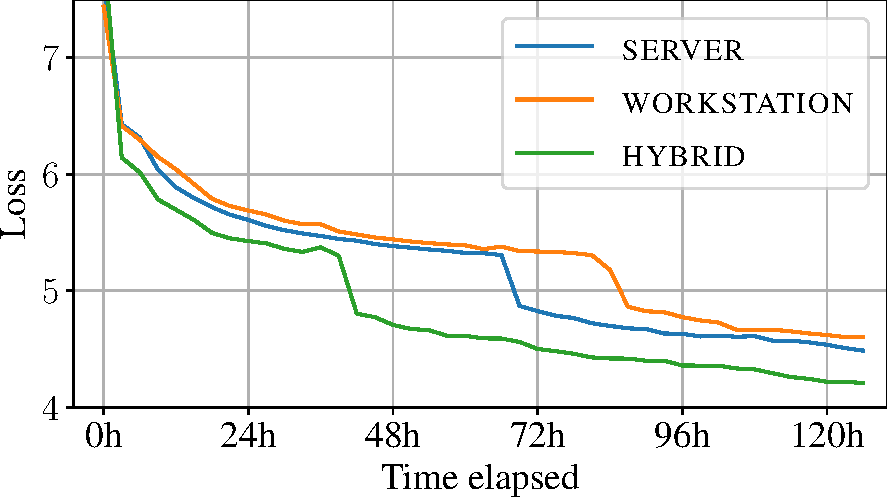
\includegraphics[height=100px]{resources/swav.pdf}
\captionof{figure}{SwAV pretraining performance.}
\label{fig:swav_perf}
\end{minipage}
\begin{minipage}[b][][b]{0.49\textwidth}
\centering
\renewcommand{\arraystretch}{1.2}
\begin{tabular}{lccc}
\toprule
\multicolumn{1}{c}{\multirow{2}{*}{Setup}} & \multicolumn{3}{c}{Algorithm} \\
 & AR & PS & Ours             \\ 
\midrule
A: 8x1Gb/s & \textbf{1.19} & 4.73 & 1.20 \\
B: 16x0.2Gb/s & \textbf{5.3} & 39.6 & \textbf{5.3} \\
C: A + B& 5.69 & 14.1 & \textbf{2.96} \\
D: B + 1x2.5Gb/s & 5.3 & 3.22 & \textbf{3.18} \\
\bottomrule
\end{tabular}
\vspace{8pt}
\captionof{table}{ResNet-50 averaging performance.}
\label{tab:averaging_perf}
\end{minipage}
\vspace{-4pt}

\subsection{Self-supervised pretraining for language understanding}
\label{sect:exp_albert}

Next, we investigate how collaborative training performs for more complex models. In this experiment, we pretrain the ALBERT-large~\cite{albert} masked language model on the WikiText-103 dataset~\cite{wikitext103}. We chose this setup for two reasons: first, ALBERT is very sensitive to the choice of hyperparameters, and specifically batch size, even more than regular Transformers~\cite{trainingtips}. This makes it easier to verify that DeDLOC can reproduce the training conditions of regular data-parallel training. Second, because of weight sharing, training ALBERT is relatively more compute- and less communication-intensive than regular BERT~\cite{bert}, which makes it possible to train with lower bandwidth.
\nocite{paszke2019pytorch}

As before, we follow the exact training configuration from the original paper, but use GPUs instead of TPUs. We use the implementation of ALBERT from the \texttt{transformers} library~\cite{wolf-etal-2020-transformers}. We run all experiments on cloud instances with Tesla T4 GPUs and report the training loss as a function of time, similarly to~\cite{lin2020multinode,switch}. In order to evaluate how DeDLOC performs with different network speeds, we consider the following setups on the same platform with controlled conditions:
\begin{itemize}[leftmargin=*]
   \item \textbf{High-bandwidth:} 16 workers, each with Tesla T4 and 25 Gb/s symmetric bandwidth;
    \item \textbf{Heterogeneous:} same, but with 4x 200 Mb/s, 8x 100 Mb/s and 4x 50 Mb/s bandwidths;
    \item \textbf{Heterogeneous + load balancing:} like Heterogeneous, but with adaptive averaging (Section~\ref{sect:method_algorithm});
    \item \textbf{Auxiliary peers:} the previous setup with 4 additional CPU-only peers at 1 Gb/s bandwidth.
    \item \textbf{Time-varying:} same as previous, but with 8 additional peers at 100 Mb/s. The extra peers are training part-time, jointly alternating between 8 hours of training and 8 hours of downtime.
\end{itemize}
\pagebreak[0]

\begin{minipage}[b][][b]{0.65\textwidth}
\centering
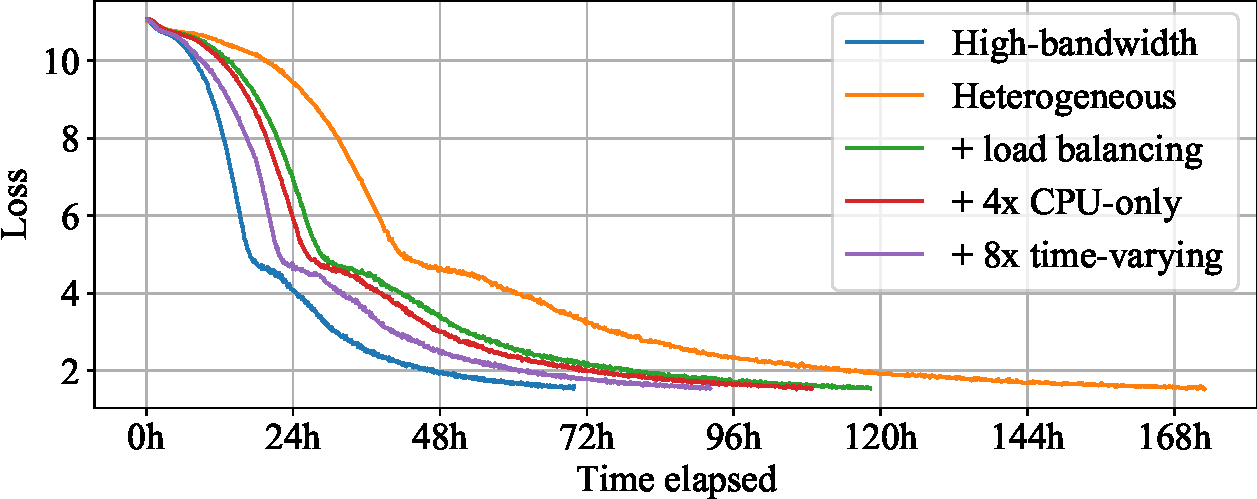
\includegraphics[width=\textwidth]{resources/convergence_albert.pdf}
\vspace{-14pt}
\captionof{figure}{ALBERT pretraining performance.}
\label{fig:albert_perf}
\end{minipage}
\begin{minipage}[b][][b]{0.32\textwidth}
\centering
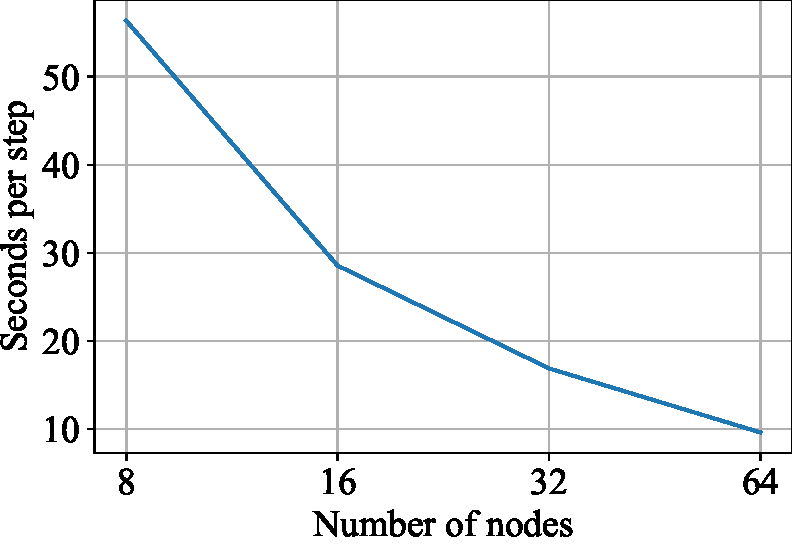
\includegraphics[width=\textwidth]{resources/albert_scalability.pdf}
\vspace{-14pt}
\captionof{figure}{Scalability measurements for ALBERT pretraining.}
\label{fig:albert_scalability}
\end{minipage}

As one can see in Figure~\ref{fig:albert_perf}, naïve training with low-bandwidth peers results in an~$\approx$ 2.5x slowdown compared to high-bandwidth ones. Enabling load balancing accelerates that setup by $\approx47\%$. This effect grows to over 60\% when adding 4 auxiliary peers. Finally, adding 8 part-time peers allows the collaboration to train at 74\% the speed of the high-bandwidth setup without sacrificing the training stability. This turns the latter setup into a viable alternative to traditional distributed training without the need for expensive infrastructure (see the cost analysis in Appendix~\ref{appendix:cost_analysis}). In addition, we demonstrate the high scalability of DeDLOC in Figure~\ref{fig:albert_scalability}, which was obtained by running the same experiment with a varying number of nodes and measuring the time between gradient descent steps. 

\vspace{-6pt}
\subsection{Real-world collaborative training}\label{sect:exp_bengali}
\vspace{-4pt}

For our final evaluation, we organized an actual collaborative training run with volunteer participants, who were asked to pretrain a Transformer masked language model for the Bengali language. This task was chosen deliberately to show the benefits of collaborative training: Bengali has over 230M native speakers who can benefit from recent advances in NLP, but there are few pretrained models available for this language.
We recruited 30 Bengali-speaking volunteers and 10 outside collaborators. All participants received instructions for contributing with free cloud platforms and access to the code for training on local computers. To avoid bias, we did not encourage any specific form of participation: volunteers were free to choose what hardware they contributed and for how long.

Specifically, we trained the ALBERT-large model on Wikipedia and the Bengali part of the OSCAR~\cite{Oscar} multilingual corpus. The model was named sahajBERT after conducting a poll among the participants. We adapted our preprocessing by following the best practices for the Bengali language described in Appendix~\ref{appendix:bn_albert_tokenizer}. To stream from a mix of Wikipedia and OSCAR, the training process iteratively sampled examples from one or the other dataset, as described in Section~\ref{sect:method_system_design}. We accounted for uneven size and quality of data by oversampling Wikipedia by a factor of 2, which resulted in mixing probabilities of 0.23 for Wikipedia and 0.77 for OSCAR. Other hyperparameters were set to the same values as in Section~\ref{sect:exp_albert}. Also, in Appendix~\ref{appendix:xl} we report the results of sahajBERT-XL --- a four times larger model with a specialized architecture that used both GPU and TPU resources.

\begin{figure}[b]
\vspace{-14pt}
% \captionsetup[subfigure]{belowskip=-1pt}
\noindent
\centering
\begin{subfigure}[t]{0.37\textwidth}
\centering
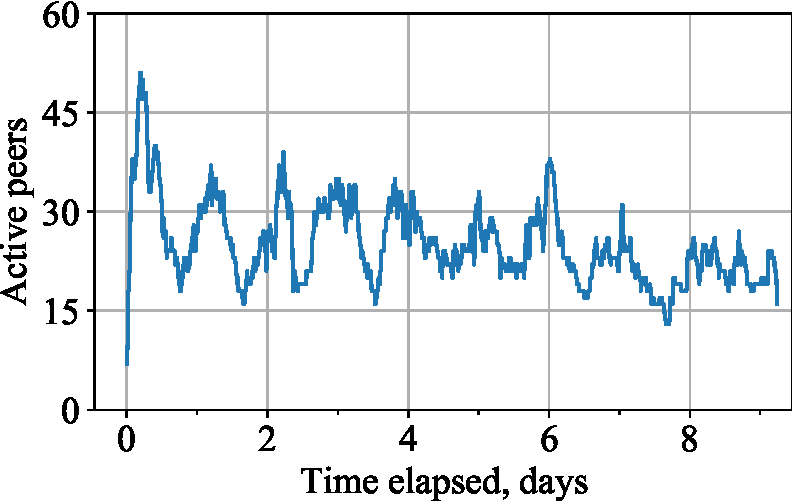
\includegraphics[width=\textwidth]{resources/peer_activity.pdf}
\caption{Collaboration activity.}
\label{fig:activity}
\end{subfigure}
\begin{subfigure}[t]{0.3\textwidth}
\centering
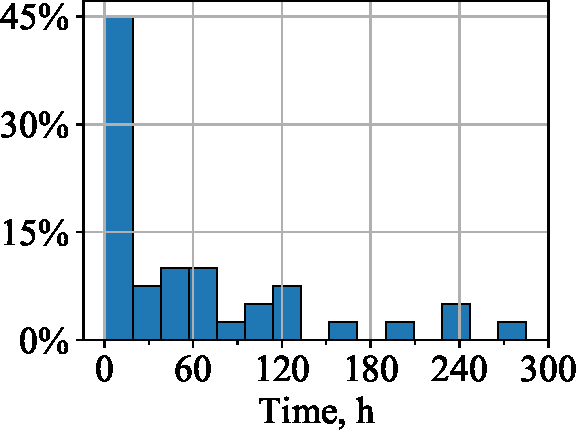
\includegraphics[width=\textwidth]{resources/contrib_hist.pdf}
\caption{Participation time histogram.}
\label{fig:contrib}
\end{subfigure}
\begin{subfigure}[t]{0.3\textwidth}
\centering
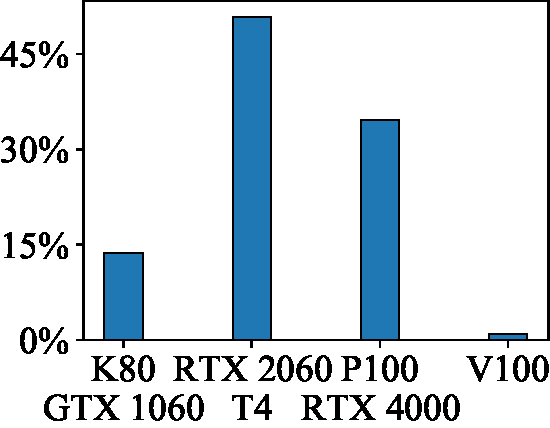
\includegraphics[width=\textwidth]{resources/gpu_hist.pdf}
\caption{Summary of volunteer hardware with example GPUs.}
\label{fig:device}
\end{subfigure}
\vspace{-4pt}
\caption{Collaborative experiment summary.}
\end{figure}


In total, the 40 volunteers contributed compute time from 91 unique devices, most of which were running episodically. Figure~\ref{fig:contrib} shows that although the median GPU time contributed by volunteers across all devices was $\approx$ 1.5 days, some participants ran the training script on several devices, attaining more than 200 hours over the duration of the experiment. With the exception of the start and the end of the collaborative run, the number of simultaneously active devices mostly varied between 15 and 35 depending on the local time. There was less activity in the last 3 days, likely because the volunteers could see that the model has converged on a public Weights \& Biases~\cite{wandb} dashboard.

As depicted in Figure~\ref{fig:device}, individual device performance varied significantly among the collaborators. Along with the resources provided by participants, we also used 16 preemptible single-GPU cloud T4 instances for training.
We have estimated that the average volunteer device consumed 6.95 GB of network traffic per hour of training. While this bandwidth usage is by no means insignificant, it is comparable with cloud gaming~\cite{google_stadia} or high-quality video streaming~\cite{netflix}.

The model converged after 8 days of training, which is 1.8x as fast as regular distributed training with 8 V100 GPUs that we ran as a baseline; Figure~\ref{fig:collab_loss} displays the convergence plots for both setups. At the same time, the stepwise learning curves of the two runs were virtually identical (see Appendix~\ref{appendix:stepwise_learning_curves}), which supports our hypothesis that training with DeDLOC is equivalent to a regular large-batch SGD.
 
\vspace{2pt}
\begin{minipage}[b]{0.49\textwidth}
\centering
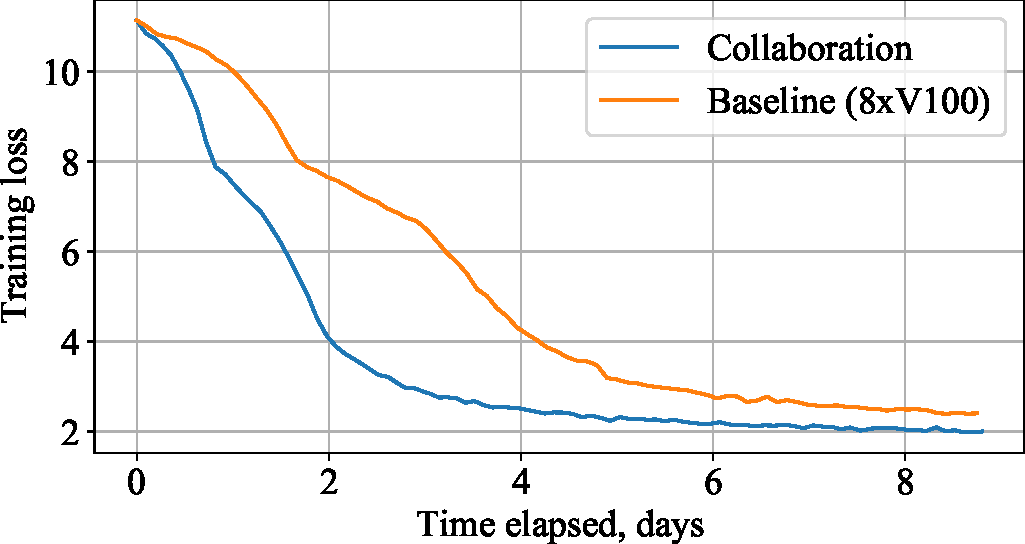
\includegraphics[width=0.95\linewidth]{resources/loss_collab_bengali.pdf}
\vspace{-4pt}
\captionof{figure}{Training progress of sahajBERT.}
\label{fig:collab_loss}
\end{minipage}
\begin{minipage}[b]{0.5\textwidth}
\setlength{\tabcolsep}{2pt}
\renewcommand{\arraystretch}{1.2}
\begin{tabular}{lcc}
\toprule
Model  & Wikiann F1 &NCC Accuracy \\
\midrule
bnRoBERTa           & 82.32 $\pm$ 0.67 &  80.94 $\pm$ 0.45 \\
IndicBERT           & 92.52 $\pm$ 0.45 &  74.46 $\pm$ 1.91 \\
XLM-R               & 96.48 $\pm$ 0.22 &  90.05 $\pm$ 0.38 \\
\midrule
sahajBERT           & 95.45 $\pm$ 0.53 &  91.97 $\pm$ 0.47 \\
sahajBERT-XL        & \bf 96.59 $\pm$ 0.26 & \bf 92.91 $\pm$ 0.43 \\
\bottomrule
\end{tabular}
\captionof{table}{Downstream evaluation results.}
\label{tab:downstream}
\end{minipage}

Finally, we compared the Bengali language representations of sahajBERT with those of other pretrained models on several downstream applications. The first model is XLM-R Large~\cite{xlmr} --- a cross-lingual Transformer-based masked language model that was pretrained on 100 languages and remains a strong baseline for multilingual representation learning. Similarly to sahajBERT, the second model, IndicBERT~\cite{kakwani-etal-2020-indicnlpsuite}, is also based on the ALBERT architecture; however, it was pretrained on 12 languages, including Bengali and Indian English. The third model, bnRoBERTa~\cite{jain2020indictransformers}, is a RoBERTa architecture trained on a monolingual Bengali corpus. We evaluate the model quality on two tasks: WikiANN~\cite{pan-etal-2017-cross} named entity recognition dataset and Soham News Category Classification benchmark from IndicGLUE~\cite{kakwani-etal-2020-indicnlpsuite}. For a detailed description of the setup, refer to Appendix~\ref{appendix:exp_bengali_evaluation}.

As shown in Table~\ref{tab:downstream}, sahajBERT performs comparably to three strong baselines despite being pretrained in a heterogeneous and highly unstable setting.
Notably, our collaboratively trained model outperforms two specialized monolingual baselines and demonstrates competitive results to XLM-R Large, even though the latter has significantly more parameters (560 million instead of 17 million) and was trained on five hundred high-performance data center GPUs instead of tens of low-cost or even free-tier accelerators.
This result confirms previous findings on the benefits of parameter sharing  that were made by authors of ALBERT. Also, it highlights one additional advantage of such architectures: specifically, one can train a high-quality representation model in a communication-constrained setting (for instance, over the Internet) without facing noticeable data transfer bottlenecks.
\section{Conclusion}

This paper introduces \textsc{Petals}, a system for efficient collaborative inference and fine-tuning of large language models. We offer a user-friendly generation interface and a flexible API to access models served over the Internet. We use 8-bit compression that reduces the resource requirements to run very large models. In addition, we develop algorithms for reliable routing and load balancing.

% Since \textsc{Petals} is open-source, we would like it to evolve based on the community's feedback, incorporating relevant research advances and adding support for features in demand.
With the release of this system, we hope to broaden access to LLMs and pave the road to applications, studies or research questions that were previously not possible or simply too expensive.

% [Commented since the Discussion section has been moved to the main text]
% Running LLMs over the Internet raises a broad range of related questions. One of them is privacy: how to avoid revealing private data to outside peers. Another challenge is to ensure that participants can benefit from this system equitably, i.e. in proportion to their contribution.
% We discuss future problems such as privacy, security, and incentive structures in Appendix~\ref{sect:discussion}.


\bibliography{custom}
\bibliographystyle{icml2023}

\appendix

\clearpage

\section*{\scalefont{1.2}Appendix}


\section{Quality and efficiency of BLOOM with 8-bit quantization}\label{appendix:8bit_quality}

\begin{table}[b]
\begin{minipage}{0.56\textwidth}
\centering
\caption{Zero-shot accuracy for \mbox{BLOOM-176B} and \mbox{OPT-175B} with 8-bit and 16-bit weights.\nocite{eval-harness}}
\vspace{9pt}
\resizebox{\linewidth}{!}{%
\begin{tabular}{lccccc}\toprule
\textbf{Model}            & \textbf{Bits} & \textbf{HellaSwag} & \textbf{LAMBADA} & \textbf{WinoGrande} & \textbf{Avg}             \\\midrule
\multirow{2}{*}{BLOOM}    & 16            & 73.0               & 67.2             & 70.1                & 70.1                     \\
                          & 8             & 72.8               & 68.1             & 70.1                & 70.3                    \\\midrule
\multirow{2}{*}{OPT} & 16            & 78.5               & 74.7             & 72.6                & 75.3                     \\
                          & 8             & 78.5               & 74.6             & 71.7                & \multicolumn{1}{r}{74.9} \\\bottomrule
\end{tabular}
}
\label{tab:quality}
\end{minipage}
\hspace{4px}
\begin{minipage}{0.42\textwidth}
\centering
\caption{Generation throughput (tokens/s) for BLOOM-176B with 8-bit and 16-bit weights on 8$\times$~A100 GPUs.}
\label{tbl:memory_footprint}
\resizebox{0.75\linewidth}{!}{%
\begin{tabular}{lccc}\toprule
\multirow{2}{*}{\bf Weights}& \multicolumn{3}{c}{\bf Batch size} \\\cmidrule{2-4} & \bf 1 & \bf 8 &\bf 32  \\\toprule
16-bit       & 4.18 & 31.3  & 100.6  \\
8-bit        & 3.95 & 29.4  & 95.8\\\bottomrule
\end{tabular}
}
\label{tab:throughput}
\end{minipage}
\end{table}

As shown in Table~\ref{tab:quality}, this method has little effect on LLM quality for major benchmarks.
In terms of inference time, Table~\ref{tab:throughput} demonstrates that quantization has about $5\%$ of overhead with batch size 1 (20 tokens), but becomes negligible for larger batches.




\section{Estimating theoretical best throughput with RAM offloading}\label{appendix:offloading_estimate}
In this estimate, we use the best possible hardware setup for offloading: CPU RAM offloading via PCIe 4.0 with 16 PCIe lanes per GPU.
In 8-bit, the model uses 1 GB of memory per billion parameters, and PCIe~4.0 with 16 lanes has a throughput of 256 Gbit/s. We assume an offloading latency of zero in the upper bound estimation. As such, offloading 176B parameters takes at least:
$$\frac{176 \text{ GB} \cdot 8}{256 \text{ Gbit/s}} = 5.5\text{ seconds}$$
This gives the upper bound of $1 / 5.5 \approx 0.18$ tokens/s for the inference speed.

\section{Extension to beam search algorithms}\label{appendix:beam_search}

There are several variations of beam-search algorithm used for language model inference, including standard beam search, diverse beam search, constrained beam search, and more. A common thread between those algorithms is that they maintain a fixed number $k$ of candidate sequences between steps. These sequences are informally referred to as the ``beam''. On every step, these algorithms generate possible continuations of sequences in the previous beam, then use some fitness criterion to select $k$ of these continuations for the next beam.

From a computational point of view, this procedure is similar to simple ``greedy'' inference with a batch of $k$ sequences. However, there is one important difference: unlike batched inference, beam search algorithms can ``shuffle'' candidate sequences between steps. In other words, 3rd best sequence from time step $t$ can produce 1st or 2nd (or any other) sequence on the next step. Furthermore, a single sequence on time step $t$ can produce multiple sequences selected for step $t+1$.

Since different beam search variantions use different criteria for selecting top sequences, we need a generic algorithm that can fit any criterion. In our system, we implement this by allowing clients to reorder server-side attention cache after each step. Formally, a client can send a list of at most $k$ integers in range $[1, k]$, where i-th index specifies which previous attention cache should be used when generating $i$-th sequence of the next beam.

For instance, when given indices $[2, 2, 1, 3, 2]$, a server will use 2nd best sequence from step $t$ to produce the new 1st, 3rd and 5th best sequences. Previous 1st and 3rd best sequences go to 3rd and 4th places, respectively. Finally, previous 4th and 5th sequences are discarded. From a technical point of view, servers implement this reordering by reordering attention cache with the specified indices (\texttt{torch.gather} operation) immediately before performing an inference step.



\section{Details of the server load balancing algorithms}\label{appendix:load_balancing_algo}

\paragraph{Measuring throughput.} Before joining for the first time, each server measures its Internet connection throughput (in tokens/second, using one of public web APIs for doing that) and GPU throughput (in tokens/second, using a small benchmark running several forward passes). The minimum of these values becomes the overall server throughput, which is then cached for future runs.

\paragraph{Initial block assignment.} We assume that each server holds a segment of \textbf{consecutive} transformer blocks to minimize inference latency. Clients may request to perform a forward or backward pass for the whole segment of blocks or its subsegment, if necessary. Normally, each server loads as many blocks as it can fit in its GPU memory, unless a user limits the number of blocks to utilize the rest of memory for something else.

Before starting, each server calculates the values of $t_i$~-- the total throughput of servers currently holding the $i$-th block or loading it (to start holding it in a few minutes). Then, to find the best segment of blocks to serve, the server looks for the most narrow bottleneck in the network. Formally, if the model has $L$ blocks and the server can hold $K$ of them in its GPU memory, we calculate:
\begin{equation}\label{eqn:load_balancing}
start=\underset{i=1}{\overset{L-K+1}{\arg\min}} \quad \mathrm{sorted}([t_i,\ t_{i+1},\ \ldots,\ t_{i+K-1}])
\end{equation}
Here, $\arg\min$ compares the sorted arrays lexicographically and chooses the leftmost $start$ in case of multiple minimums.

This way, the next joining server would always cover a block with the smallest $t_i$. If there are multiple bottlenecks like this, the server will try to cover as many of them as possible (we choose to cover the minimums first because the overall throughput is the minimum of throughputs among model blocks). Among the remaining options, we choose a segment covering as many second minimums as possible, and so on.

\paragraph{Quality of block assignment.} While we are not aware of the exact polynomial-time solution for the problem of assigning the segments optimally, we have conducted computational experiments and found out that this greedy algorithm (running in polynomial time) usually finds an assignment with total throughput of 90-100\% of the optimal one (found by trying out all possible assignments in exponential time), given that the values of throughput are realistic to our setup.

\paragraph{Rebalancing.} Since servers may leave at any time, each server also periodically checks if the current assignment is "good enough" compared to the throughput estimated by running the greedy solution for servers currently present in the network.

Formally, each server periodically looks for a segment of blocks that is more appropriate than the currently loaded blocks with respect to the $\arg\min$ rule~(\ref{eqn:load_balancing}). If it finds one, it simulates how the rest of the servers would behave if we replace the current blocks with the new ones (how other servers would change their blocks afterwards). If the eventual throughput is at least $p\%$ better, the server commits to the change and announces that it changes the blocks, then other servers do the rest of the changes (eventually increasing the total throughput).

We use $p=20\%$ since it gives a reasonable trade-off between the swarm throughput and the frequency of block replacements in our experiments (see Appendix~\ref{appendix:load_balancing_exps}). Specifically, a lower value of $p$ leads to block replacements happening too often, which negatively affects the inference latency since each block replacement resets attention caches for this block.

\paragraph{Stability of the greedy algorithm.} The rebalancing algorithm does not cause oscillations since a series of block replacements is executed only if it leads to eventually increasing throughput by at least $p\%$. Once a "good enough" throughput is achieved, servers do not change their blocks anymore (unless an essential number of servers join or leave). We verified this behavior computationally, simulating a network with thousands of servers with different throughputs.

To conclude, this greedy heuristic allows servers to quickly close the gaps if a substantial share (up to 100\%) of servers holding certain blocks leave, but avoids excess block replacements otherwise.

\begin{figure*}[tb]
    \centering
    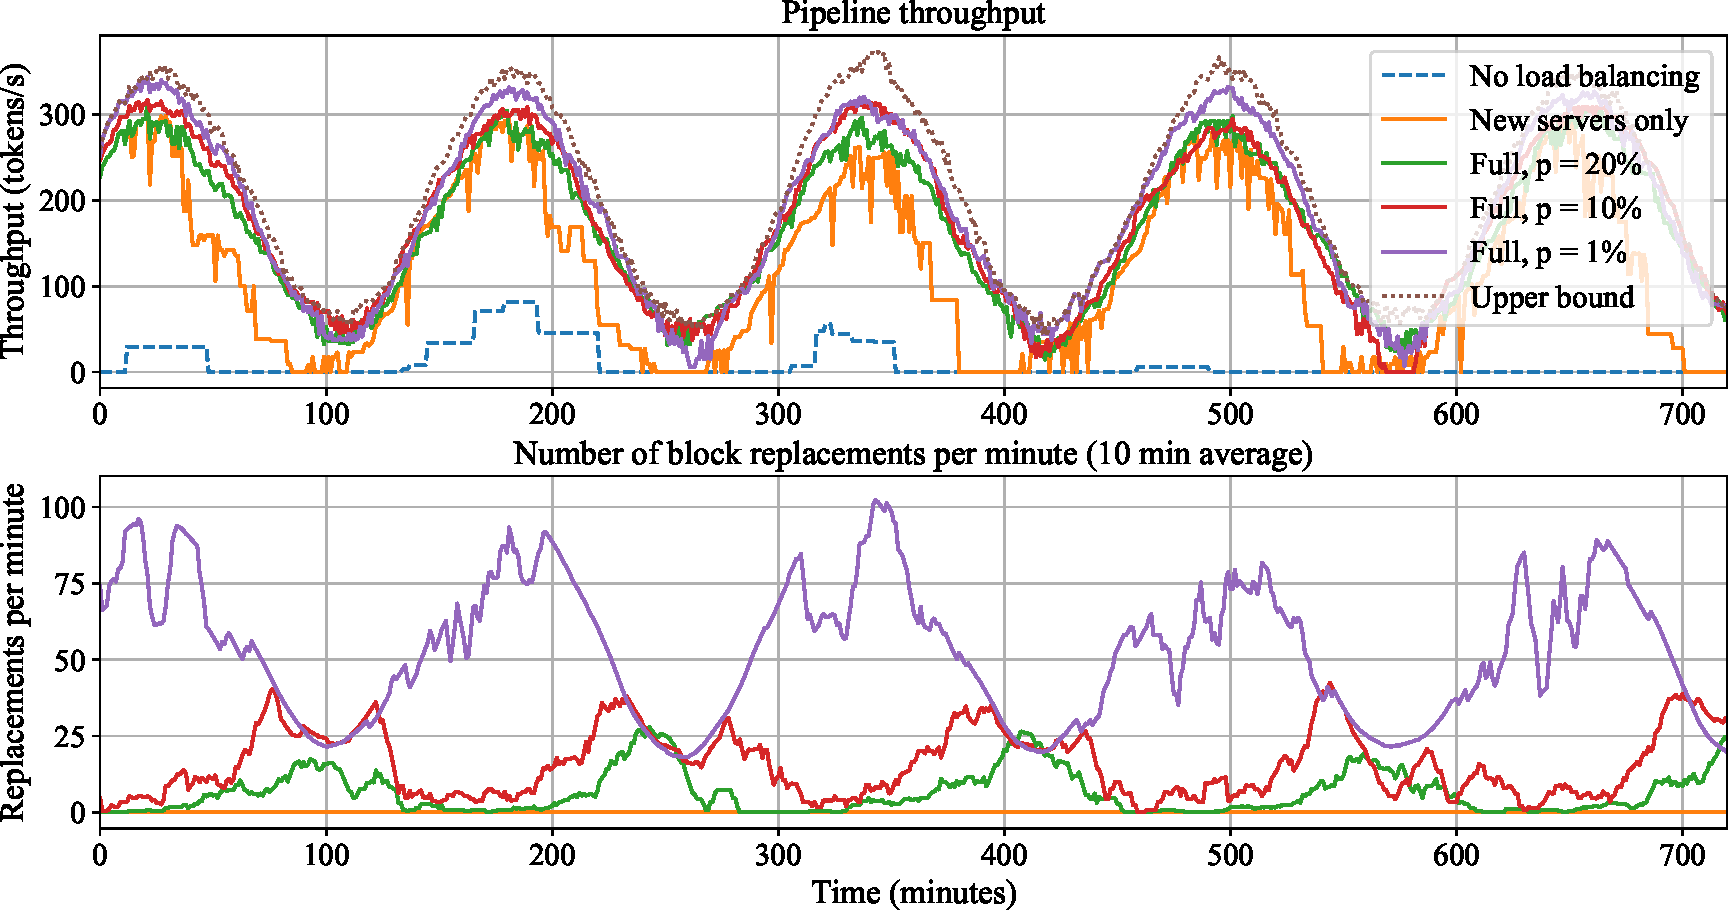
\includegraphics[width=\linewidth]{resources/load_balancing_exps.pdf}
    \vspace{-12pt}
    \caption{Behavior of the load balancing algorithms evaluated in Appendix~\ref{appendix:load_balancing_exps}.}
    \label{fig:load_balancing_exps}
    \vspace{-6px}
\end{figure*}


\section{Evaluation of the server load balancing algorithms}\label{appendix:load_balancing_exps}

In this section, we measure the effectiveness of the load balancing algorithm used in our system. We run all experiments using a fleet of 206 virtual instances that simulate participants. To keep experiment costs manageable, we do not use GPUs for this evaluation, instead simulating uneven server throughput programmatically. For each server, we sample its throughput from the uniform distribution $t \sim \mathbb{U}[0, 100]$ tokens/second, then sample its memory size so it can hold $b \sim \mathbb{U}[1, 10]$ blocks (out of 70 blocks in total, as in BLOOM-176B).

Each server follows a certain availability schedule, i.e. turns on and shuts down at the same predefined time across all experiments.
We assign these schedules such that the number of active servers follows a sine wave, simulating daily activity cycles.
The schedule has approximately 100--110 active servers during peak activity and 15--25 servers at its lowest points.
Note that each peak contains a different subset of 100--110 active servers out of 206 instances in total.

We evaluate the following approaches to load balancing:
\begin{enumerate}
  \vspace{-1px}
  \item \textbf{No load balancing} -- a baseline system where servers load a random contiguous interval of model blocks.
  \vspace{-1px}
  \item \textbf{Balancing new servers only} -- a simplified load balancing where servers choose the optimal blocks when joining the swarm (using the rule~(\ref{eqn:load_balancing}) from Appendix~\ref{appendix:load_balancing_algo}) but never change them.
  \vspace{-1px}
  \item \textbf{Full load balancing} -- the full algorithm, where every minute each server checks if they need to replace their blocks. We use the efficiency threshold $p$ (as described in Appendix~\ref{appendix:load_balancing_algo}) to avoid excess block replacements.
  \vspace{-1px}
  \item \textbf{Upper bound} --- the best-case throughput estimate that reassigns contiguous block segments to servers optimally every minute.
  \vspace{-1px}
\end{enumerate}

We report their behavior in Figure~\ref{fig:load_balancing_exps}. The full load balancing maintains connectivity throughout the experiment and achieves throughput close to the upper bound (staying within the 10--15\% range most of the time). Higher thresholds $p$ perform slightly worse during peak times but require only relatively infrequent block replacements, unlike the case with $p=1\%$. Note that using the assignment leading to the upper bound is not possible in practice since it requires each server to load a different set of layers every minute, on top of solving the computationally expensive optimization problem.

Curiously, the baseline running load balancing for \textit{new servers only} achieves reasonable throughput during periods where servers are actively joining. However, it quickly loses throughput when random servers leave, since this creates ``bottlenecks'' in the pipeline that require rebalancing of existing peers. Finally, the naive baseline with random layer assignment has zero throughput most of the time because it is unable to form a complete pipeline.

\section{Experiments with a wider range of failure rates}\label{appendix:failure_rate_plots}

In this section, we follow the setup from Section~\ref{sect:experiments_basic} and provide additional evaluations for a wider range of failure rates (up to 5\%) and sequence lengths (up to 2048 tokens). The results are shown in Figure~\ref{fig:failure_rate_plots}. Unlike baselines, our algorithm provides reasonable performance \textit{in all tested conditions}, especially for higher failure rates common for communicating over the Internet, using spot/preemptible instances or unreliable hardware).

\begin{figure}[H]
    \centering
    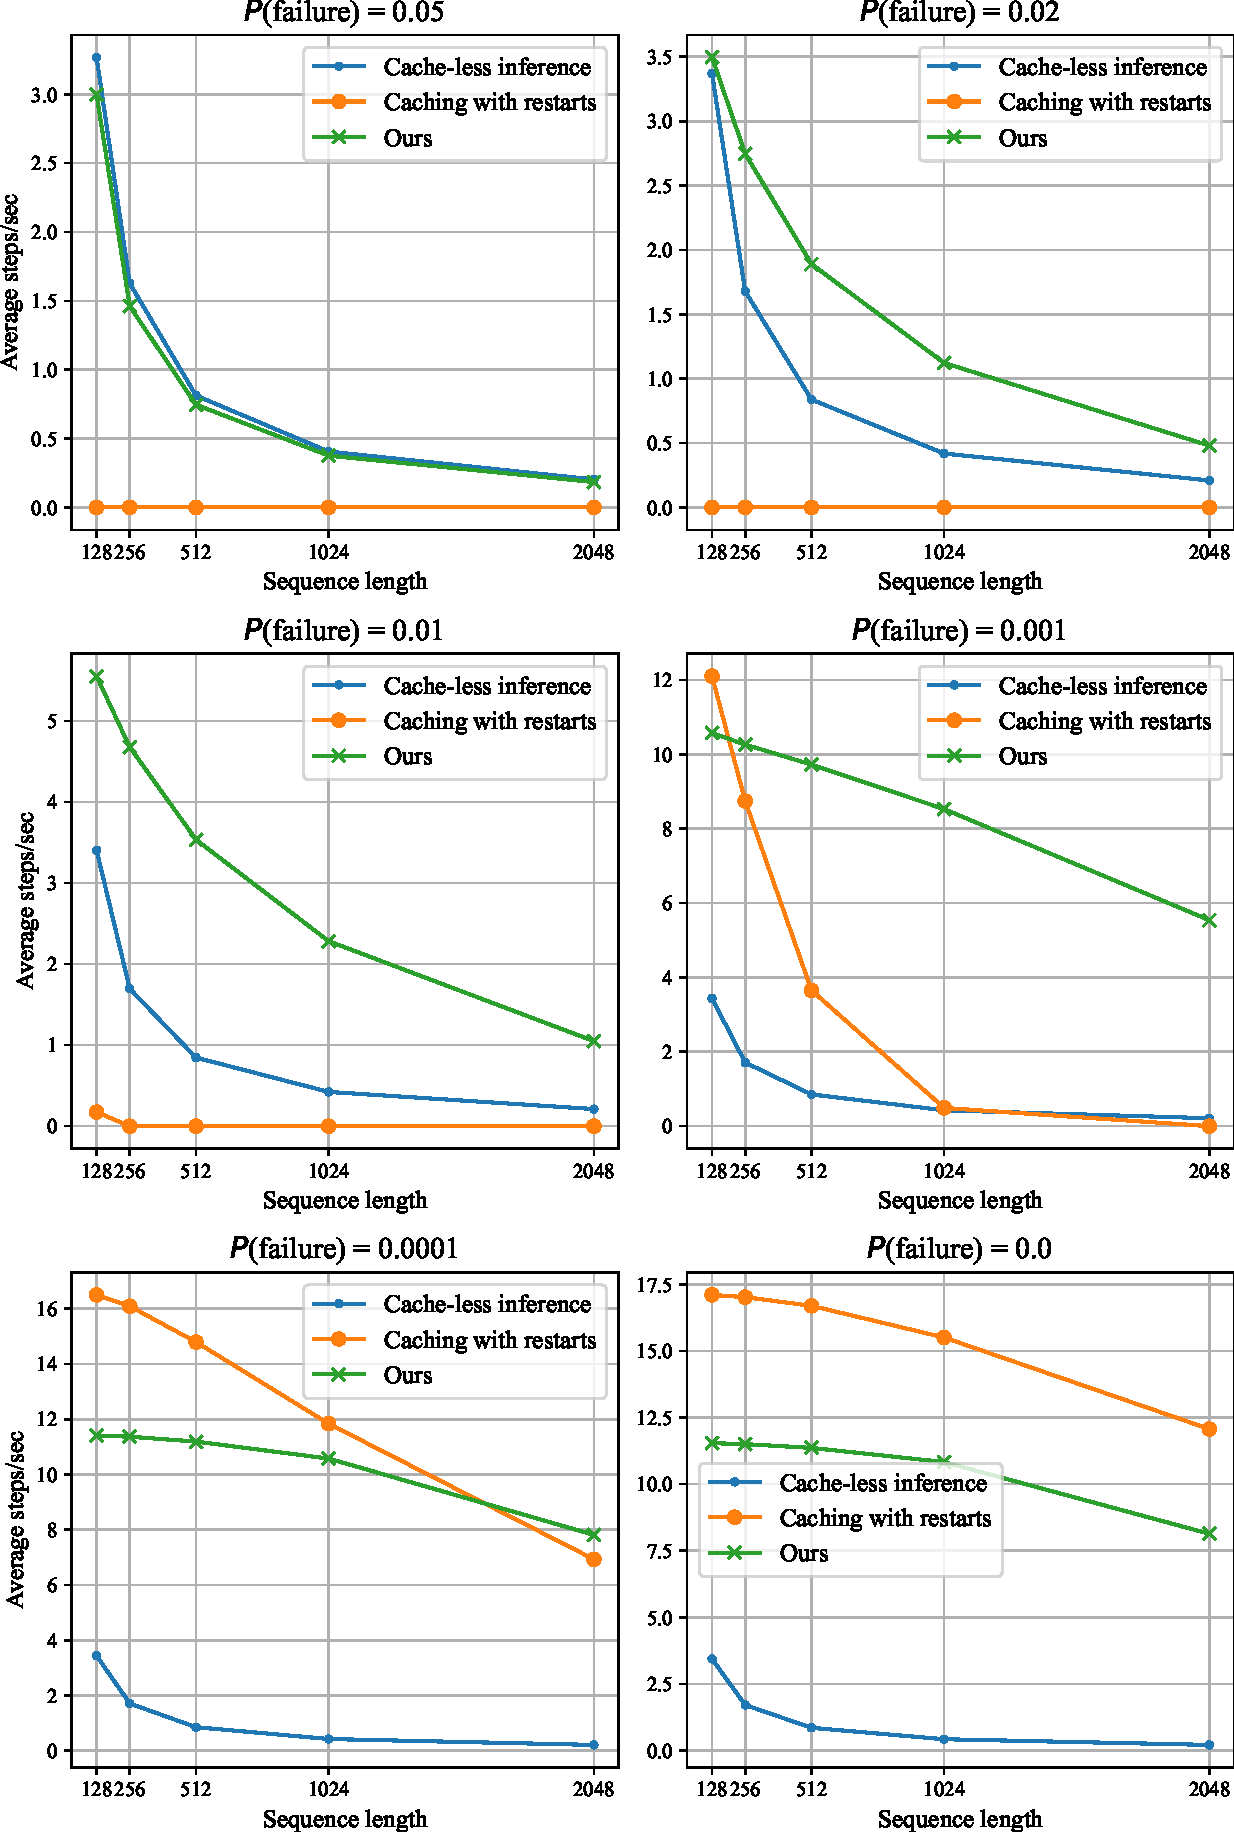
\includegraphics[width=0.875 \linewidth]{resources/pretty_failure_rate_plots.pdf}
    \caption{Sequential inference speed (steps/s) for BLOOM (7.1B) with varying failure rates. The setup is the same as in Section~\ref{sect:experiments_basic}. A failure rate $p$ means that sending a set of activations to the next pipeline stage fails with probability $p$. Zero speed means that the baseline did not finish within 1 hour.}
    \label{fig:failure_rate_plots}
\end{figure}

\section{Performance of training-time forward and backward passes}\label{appendix:backward_pass}

In this section, we evaluate throughput of training-time forward and backward passes and study factors that affect their performance. We will only consider BLOOM-176B and the ``3$\times$ A100, 1~Gbit/s'' setup from Section~\ref{sect:experiments_controlled} and focus on finetuning-specific hyperparameters, since the influence of network bandwidth and latency has already been discussed in the main paper.

\paragraph{Sequence classification.} First, we consider fine-tuning the model on a binary classification task. We take BLOOM-176B, replace the logit layer with a trainable classification head (similar to \texttt{transformers.BloomForSequenceClassification}), and add trainable prompts before the input sequence, then train the model on batches of 128-token sequences. We try \textbf{(a)} both prompt tuning and prefix tuning (involving ``deep'' prompts), \textbf{(b)} two batch sizes (8 and 32), and \textbf{(c)} two prompt lengths (16 and 4). The client shares 8 CPU cores with one of the servers and does not use the GPU.

The results are provided in Table~\ref{tbl:exp_full_step}. The prefix tuning turns out to be slower, since it adds several times more trainable parameters. Increasing prompt length and decreasing batch size also make training slower. Notably, we observe that moving client-side computations to GPU does not visibly improve performance, since the client does not perform any heavy operations in this setup\footnote{In case of sequence classification, the heaviest operation the client does is multiplying $2 \times h$ and $h \times b$ matrices, where $h$ is the hidden dimension (14336 in BLOOM-176B) and $b$ is the batch size.}.

\paragraph{Language modeling.} Next, we consider fine-tuning the model on a causal language modeling task. We take BLOOM-176B, keep the logit layer, and add trainable prompts before the input sequence. We explore the same hyperparameters as with sequence classification.

We observe that the throughput of the GPU-enabled client is similar (within 10\% difference) to the throughput in case of sequence classification, reported in Table~\ref{tbl:exp_full_step}. Indeed, the client performs only a small share of GPU computations in the forward and backward passes, and a particular model head and a loss function do not have decisive influence on the performance. However, performance of the CPU-only client turns out to be 5-10 times worse in this setup, since the client has to multiply the output embedding matrix to the hidden states of all tokens in the batch. This operation is too large to be efficiently computed on CPU\footnote{In case of language modeling, the client has to multiply $d \times h$ and $h \times b$ matrices, where $d$ is the token vocabulary size (250880 in BLOOM-176B). This is $\approx 10^5$ times more FLOPS than used in case of sequence classification.}.

\begin{table}[tb]
  \centering
 \caption{Throughput (tokens/sec) of forward and backward passes for different tasks, batch sizes, prefix lengths.}
 \label{tbl:exp_full_step}
\setlength{\tabcolsep}{3pt}
\begin{tabular}{ccccc}\toprule
\multirow{2}{*}{\bf{Mode}} & \multirow{2}{*}{\bf{Batch size}} & \multirow{2}{*}{\bf{Prompt length}} & \bf{Forward pass} & \bf{Backward pass} \\
& & & \bf{throughput}  & \bf{throughput} \\
\midrule
\multirow{4}{*}{Prompt tuning}
& 8 & 16 & 195.6 & 57.4 \\
& 8 & 4 & 213.2 & 60.8 \\
& 32 & 16 & 272.6 & 82.8 \\
& 32 & 4 & 293.1 & 84.7 \\
\midrule
& 8 & 16 & 111.0 & 42.0 \\
Prefix tuning & 8 & 4 & 178.7 & 57.8 \\
(i.e., ``deep'' prompt tuning) & 32 & 16 & 164.1 & 64.4 \\
& 32 & 4 & 255.8 & 84.8 \\
\bottomrule
\end{tabular}
\end{table}











\section*{Broader Impact}
\label{sect:broader}
\vspace{-4px}

The approach proposed in this work is only a prototype with limited direct consequences, but the long-term goal of training huge models with volunteer computing can have a lasting effect on both the research community and the general public.

\vspace{-6px}
\subsection*{Funding bias vs crowdsourcing bias} 
\vspace{-6px}
The main positive outcome we pursue is to let researchers harness volunteer computing and train models on the scale currently available only to large corporations. Ideally, a deep learning researcher with a promising idea will be able to amass the computation needed to realize this idea by involving volunteers. However, the project's appeal for volunteers depends on many factors such as subject area, current societal trends, and even researcher's personality.

For example, a project about teaching agents to play games~\cite{lc0} or fighting global pandemics~\cite{folding_covid} is likely to attract more resources than deep learning applied to soil science. In essence, volunteer computing is biased towards exciting or socially relevant research the same way as traditional HPC is biased towards the interests of those who fund it.

\vspace{-6px}
\subsection*{Alternative use and misuse} 
\vspace{-6px}
The proposed technology can be used with different economic models. If a deep learning system is immediately useful (e.g. for machine translation, information retrieval, etc), the participants could use it for their needs based on their contributions to training. This can take many forms: several labs combining their hardware and training larger models; a web-service that lets people contribute their compute instead of using ads/subscriptions; or simply a framework that someone can use to run distributed training across two or more datacenters.

Unfortunately, this also allows several opportunities for malicious use. If a machine is hacked, the attacker can use its compute unnoticed by the machine owner --- much the same way that botnets are currently used to mine cryptocurrencies. Furthermore, due to decentalized nature even legitimate Learning@home projects can be hijacked by hackers.

\vspace{-6px}
\subsection*{Security} 
\vspace{-6px}
Using crowdsourced hardware makes Learning@home susceptible to attacks from malicious participants. There are multiple attack vectors already known in P2P community: denial of service attacks, Sybil attacks, Eclipse attacks and more \cite{urdaneta2011survey, sybil_attacks_dht, dos_resistance, sybil_nodes}. Fortunately, there are variations of the DHT protocol that make it resistant to said attacks: if a reader wishes to learn more about DHT security, we recommend starting with \cite{urdaneta2011survey}.

Another source of vulnerability stems from the sequential nature of neural networks. If a single expert were to return incorrect (e.g. NaN) outputs or gradients, it could compromise the outputs of the entire network and even poison adjacent nodes through backpropagation. Recent studies expose similar attack patterns on federated learning systems \cite{bagdasaryan2018backdoor, bhagoji2018analyzing}.

The redundant nature of mixture-of-experts layers provides some degree of resistance against those attacks. A single malicious expert will only affect a small fraction of inputs that pass through this specific expert. Furthermore, a trainer with access to predictions from multiple experts could provide a higher degree of robustness by using statistical techniques (e.g., by ignoring outlier gradients). However, such techniques need to be carefully designed so as not to introduce harmful side effects.

\vspace{-6px}
\subsection*{The burden on the network} 
\vspace{-6px}
Finally, we would like to point out the potential harm that our approach can do to network infrastructure. The experiments we ran in Section \ref{sect:exp_throughput} saturate with the bandwidth of $100-200$Mbps, most of which is tensors passed between experts and trainers. 

This coincides with the typical home internet speed available in major cities of developed countries. However, not all ISPs design their infrastructure for users who always use up all their bandwidth. If too many Learning@home participants are located in one LAN or MAN, it can cause congestion or even failures in the network infrastructure. 

Similar situations frequently took place in late 2000s due to growing popularity of BitTorrent for file sharing. Fortunately, the network infrastructure is continually improving, which leads us to believe that this problem will eventually be solved. Until then, we describe several ways to reduce network load of Learning@home in Appendix E.

















\end{document}